

%
%  HBCmain
%
%  Created by Steven James Dean Martell on 2011-09-27.
%  Copyright (c) 2011 UBC Fisheries Centre. All rights reserved.
%
\documentclass[12pt]{article}

% Use utf-8 encoding for foreign characters
\usepackage[utf8]{inputenc}

% Setup for fullpage use
\usepackage{fullpage}
\usepackage{url}
\usepackage{rotate}
\usepackage{rotating}

% Uncomment some of the following if you use the features
%
% Running Headers and footers
%\usepackage{fancyhdr}
% Multipart figures
%\usepackage{subfigure}
% Natbib package for bibliography
\usepackage[round]{natbib}

% More symbols
\usepackage{amsmath} 
\usepackage{amssymb} 
\usepackage{latexsym}

% Surround parts of graphics with box
\usepackage{boxedminipage}

% Package for including code in the document
\usepackage{listings}

% If you want to generate a toc for each chapter (use with book)
\usepackage{minitoc}

% This is now the recommended way for checking for PDFLaTeX:
\usepackage{ifpdf}

%% The following is used for tables of equations.
\newcounter{saveEq} 
\def\putEq{\setcounter{saveEq}{\value{equation}}} 
\def\getEq{\setcounter{equation}{\value{saveEq}}} 
\def 
\tableEq{ 

% equations in tables
\putEq \setcounter{equation}{0} 
\renewcommand{\theequation}{T\arabic{table}.\arabic{equation}} \vspace{-5mm} } 
\def\normalEq{ 

% renew normal equations
\getEq 
\renewcommand{\theequation}{\arabic{section}.\arabic{equation}}}

\def\puthrule{ 

%thick rule lines for equation tables
\hrule \hrule \hrule \hrule \hrule} 
\usepackage{multicol}

%\newif\ifpdf
%\ifx\pdfoutput\undefined
%\pdffalse % we are not running PDFLaTeX
%\else
%\pdfoutput=1 % we are running PDFLaTeX
%\pdftrue
%\fi
%\ifpdf 
%\usepackage[pdftex]{graphicx} \else 
%\usepackage{graphicx} \fi 
\usepackage{graphicx}
\title{Estimates of population status of humpback chub (\textit{Gila cypha}) in the Grand Canyon based on a length-based mark-recapture assessment model.} 
\author{ Steven J. D. Martell\\
UBC Fisheries Centre,\\
2202 Main Mall,\\
Vancouver, BC\\
V6T 1Z4,\\
CANADA }

\date{2011-09-27}

\begin{document}

\ifpdf \DeclareGraphicsExtensions{.pdf, .jpg, .tif} \else \DeclareGraphicsExtensions{.eps, .jpg} \fi

\maketitle 
\begin{abstract}
	A length-structured population model that incorporates mark-recapture data was developed to estimate abundance of humpback chub (\textit{Gila cypha}) in the Grand Canyon between 1989 and 2011. The model was fit to observations on catch-at-length and capture-recapture data from sampling programs that employed a variety of gear types including electrofishing, tramel netting, and hoop nets. Previous assessment models were age-based and have been shown to produce biased estimates of recent recruitment estimates. The age-structured model was also limited to data on fish that were greater than 150mm total length; the minimum size required for tagging. The length-structured model developed here makes no assumptions about age of individual fish and is also fit to catch-at-length data for fish that are too small to tag. Model outputs are based the number of fish greater than a specified size, or in a fixed size interval, there are no age-based results. 
\end{abstract}

\tableofcontents

\section{Introduction}\label{sec:Intro}

In this report, I develop a length-structured mark-recapture model (hereafter, LSMR) where the accounting system for population numbers is based purely on length. The model is a statistical catch-at-length model, where the initial length distribution and recruitment each year are treated as latent variables to be estimated by fitting the model to a series of catch-at-length observations take over a period of time. A separable function is developed to estimate the year and size effect in observed catch-at-length data. The statistical nature of the model is very similar to that of \cite{fournier1982general}, but is based on catch-at-length rather than catch-age data. The model is also fit to length-based capture-recapture data, where the growth and survival of tagged animals is updated at each time step and the predicted ratio of marked and unmarked fish-at-length is used to estimate the length-based recapture rates.

%!TEX root = /Users/stevenmartell/Documents/CONSULTING/HumpbackChub/HBC_2011_Assessment/WRITEUP/HBCmain.tex
\section{Methods} % (fold)
\label{sec:methods}

There are two major methodological components in this length-based model: (1) the development of an individual based model (IBM) for simulating a capture recapture program, and (2) a statistical catch-at-length mark-recapture model to estimate the number of individual fish in each length-class in each sampling year.  A detailed description of the IBM simulation model is provided in the appendix; in short, this simulation model generates a matrix of the number of fish captured-at-length, a matrix of the number of newly marked fish released-at-length, and a matrix of marked fish recaptured-at-length.  The remained of this section is a detailed analytical description of the statistical catch-at-length model used to estimate the abundance-at-length of humpback chub in the Grand Canyon.

The following is a description of the analytical model for the length-structured mark-recapture model (hereafter, LSMR) used in this assessment.  I present the analytical model in the form of a table (Table \ref{table:LSMRmodel}) where the order in which model equations are presented also represent the order in which the calculations proceed in the computer code.  Equations presented in each table are referenced, for example, as \eqref{eq:T1.1}, where the T1 refers to Table \ref{table:LSMRmodel}, and the .1 refers to the first equation in that table. The LSMR model was implemented in AD Model Builder \citep{fournier2011ad}, and the template code is available in the appendix of this document as well as a Git code repository (\url{https://code.google.com/p/lsmr-project/}).  The description of the Length-Structured Mark-Recapture (LSMR) model is broken down into: input data, estimated parameters, dynamics of numbers-at-length, capture probability, and negative log-likelihoods and prior densities.

The following notation is used to define the dimensions of various variables. Vector quantities are designated with an an arrow ($\vec{x}$) or with a single subscript, and matrix is denoted by boldface uppercase letters ($\mathbf{X}$) and where two subscripts are shown denotes the element specific calculation.  Higher dimensional arrays are indicated by normal upper case letters with 3 or more subscripts.  

\subsection{Input data} % (fold)
\label{sub:input_data}
The model dimensions consists of time intervals (year indexed by $i$) and length intervals (index by $j$, \ref{eq:T1.1}).  Capture-recapture data for the humpback chub have been collected on an annual basis since May 1, 1989,  and the latest capture record in this analysis is February 27, 2012.  The principle input data for LSMR consists of model dimensions (e.g., years, length intervals $\Lambda$), a matrix of catch-at-length data $\mathbf{C}$ for each year, the number of new marks released-at-length $\mathbf{M}$, and the number of recaptured marks-at-length $\mathbf{R}$.


\subsubsection{Processing length frequency data} % (fold)
\label{ssub:processing_length_frequency_data}
At the time of writing this report, there were a total of 81,812 records in the database for humpback chub, of which 35,696 are unique individuals (some of which may occur in the database only once).  Details on the construction of Tables \ref{table:Captures}--\ref{sidewaystable:Recapture_GILL} can be found in Appendix \ref{sec:processing_mark_recapture_by_length_information}. In short, the length composition and mark-recapture information, along with summary statistics about the number of trips, days fished and other units of effort were obtained.

The length composition of the newly marked and recaptured individuals each year were compiled in tables (Appendix \ref{sec:processing_mark_recapture_by_length_information}) and bar charts to characterize recruitment and growth of newly marked and previously marked HBC, respectively.
% subsection processing_length_frequency_data (end)
% subsection input_data (end)

\subsection{Estimated parameters \& parametric functions} % (fold)
\label{sub:estimated_parameters}
An array of estimated parameters \eqref{eq:T1.5} is denoted by $\Theta$ and consists of 9 +$(2I-1)$ +$J$ unknowns, where $I$ is the total number of time steps (years) and $J$ is the total number of length intervals.  

Natural mortality is a function of length \eqref{eq:T1.6}, where the natural mortality at the asymptotic length $M_\infty$ is estimated from the data.   Note that in \eqref{eq:T1.6} the estimated natural mortality rate is confounded with asymptotic length $l_\infty$ which is also an estimated parameter along with the von Bertalanffy growth coefficient $k$. Selectivity is also assumed to be a parametric function of length \eqref{eq:T1.7} where $l_x$ and $g_x$ represent length-at-50\% vulnerability and the standard deviation of the logistic function, respectively.  
% subsection estimated_parameters (end)

\subsection{Growth transition} % (fold)
\label{sub:growth_transition}
The growth parameters are used to calculate a vector of growth increments $\vec{\Delta}$ assuming von Bertalanffy growth \eqref{eq:T1.8}. An additional parameter $\beta$ is used to characterize the variability in annual growth increments for individual fish.  The asymptotic length $l_\infty$ is defined as the average asymptotic length for a population of fish.  It is assumed in \eqref{eq:T1.8} that individuals greater than $l_\infty$ continue to grow at a much reduced rate $k$; this is accomplished by exponentiating the growth increment equation ($(l_\infty-x_j)(1-\exp(-k\tau))$), adding 1.0, and taking the natural logarithm ensuring that \eqref{eq:T1.8} remains positive for all positive values of $l_\infty$, $k$, and $\Lambda$.

The model assumes that the distribution of size transitions from length bin $x_j$ to subsequent length bins $x_j'$ follows a gamma distribution \eqref{eq:T1.9}. The mean of this function is denoted by the growth increment ($\Delta_j$) and a variance equal to $\Delta_j \beta$.  Each row of the size transition matrix $\mathbf{P}$ is normalized to sum to 1.0, and $\mathbf{P}_{j,j'}=1.0$ when $j=j'=J$, where $J$ is the number of length intervals (i.e., individuals in the last length interval represent a plus group).

There is also an alternative to jointly estimating a size transition matrix based on mark recapture data.  A series of size transition matrices based on annual growth increments for humpback chub captured and recaptured in the subsequent year was also constructed. Details are outlined in Appendix \ref{sec:size_transition_matrix_from_mark_recapture_data}.

% subsection growth_transition (end)

\subsection{Size distribution of new recruits} % (fold)
\label{sub:size_distribution_of_new_recruits}
Newly recruiting individuals at each time step are assumed to have a distribution of lengths that follows a gamma distribution \eqref{eq:T1.10}, where $\vec{p}$ represents the probability of a new recruit being in size interval $x_j$. Two parameters ($\mu$ and $\sigma$) corresponding to the mean and the coefficient of variation of the gamma distribution, respectively, are jointly estimated in the model.  Note that the vector $\vec{p}$ is also normalized to sum to 1.0.
% subsection size_distribution_of_new_recruits (end)

\subsection{Initial states} % (fold)
\label{sub:initial_states}
A matrix of the total numbers-at-length in a given time step is denoted by $\mathbf{N}$, and the total number of marked individuals at large is denoted by $\mathbf{T}$, \eqref{eq:T1.11}.  To initialize the vector of numbers-at-length in the initial year ($i=1$), a $J$ by $J$ matrix of recruits prior to the initial year $\mathbf{R}$ is constructed using \eqref{eq:T1.12}, where $\ddot{R}$ and $\vec{\eta}$ is an estimated scaler and vector respectively.  Note that the additional constraint  of $\sum_j \eta_j = 0$ is also required to properly estimate the scaler $\ddot{R}$.

The initial numbers-at-length in the initial year is based on the recursive equation defined by \eqref{eq:T1.13}.  This recursion occurs $J$ times where the initial recruits in the first iteration survive at a rate $\exp(-\vec{m})$ and then grow based on the size transition matrix $\mathbf{P}$.  In the second recursion, the next vector of new recruits is added and the survival and growth repeats.  Note that if $\vec{\eta}=0$, then a stable size distribution is set up based on the natural mortality, size transition and initial recruitment.  The addition of $\vec{\eta}$ allows for a no stable size distribution to be set up in the initial year.
% subsection initial_states (end)

\subsection{Dynamics of numbers-at-length} % (fold)
\label{sub:dynamics_of_numbers_at_length}
The size transition matrix $\mathbf{P}$ is the key component when modelling a population using length and not age. First, a matrix of annual recruits distributed over size intervals based on $\vec{p}$ is constructed in \eqref{eq:T1.14}, where $\bar{R}$ is the average recruitment over all years except the initial year, $\vec{\nu}$ is a vector of annual recruitment deviates.  The  vector of numbers-at-length in the next time step $\tau$ is given by \eqref{eq:T1.15}, where $\vec{R}_i$ is the corresponding row of recruitment from \eqref{eq:T1.14}.
% subsection dynamics_of_numbers_at_length (end)

\subsection{Capture probability} % (fold)
\label{sub:capture_probability}
Capture probability of fully selected fish at each time step is an unknown parameter to be estimated from the data.  A total of $I+1$ capture probability parameters are estimated \eqref{eq:T1.16}, where $\bar{f}$ is a scaler and $\vec{\zeta}$ is a vector of annual deviates with the constraint $\sum_i \zeta_i = 0$. 
% subsection capture_probability (end)

\subsection{Predicted captures and recaptures} % (fold)
\label{sub:predicted_captures_and_recaptures}
Predicted captures of unmarked and marked fish are based on the average number of fish available over each time step.  The total number of marked and unmarked fish captured at each time step $\tau$ is denoted by $\hat{C}$, and in \eqref{eq:T1.17} no additional mortality associated with handling and tagging unmarked fish was assumed. Handling mortality could easily be incorporated into the catch equations, however, it is completely confounded with the capture probability and in this case not estimable without additional information.  The predicted number of recaptured individual fish ($\mathbf{R}$) is based on the same catch equation \ref{eq:T1.18} and an estimate of the total number of tags at large ($\mathbf{T}$).  For the initial time step, the total number of tags at large is $\mathbf{T}=0$, as no fish have been tagged.  For time steps greater than 1, the total number of tags at large is based on the recursive survival, growth and recruitment of newly marked animals ($\mathbf{M}$).  This recursive equation is defined by \eqref{eq:T1.20}, where it is assumed that tagged and untagged individuals have the same natural mortality rate and size transition matrix.  The number of newly marked fish at each time step is based on the difference between the total catch and number of recaptured fish in the total catch \eqref{eq:T1.19}.
% subsection predicted_captures_and_recaptures (end)

\begin{table}
  \centering
\caption{Data, parameters, and analytical procedures for the length-based mark-recapture model.}\label{table:LSMRmodel} 
\tableEq
	\begin{footnotesize}
    \begin{align}
        \hline
		&\mbox{INDEXES, DATA \& CONSTANTS} \nonumber\\
		&\mbox{index for time, index for length interval} 
		&i,j 
		\label{eq:T1.1}\\ 
		&\mbox{time step}  & \tau 
		\label{eq:T1.2}\\
		&\mbox{set of midpoints of length intervals}
		&\Lambda = \{x_1, \ldots,x_J\}
		\label{eq:T1.3}\\
		&\mbox{catch, new marks, recaptures} 
		&\mathbf{C}, \mathbf{M}, \mathbf{R}
		\label{eq:T1.4}\\[1ex]
		%%
		%%
		&\mbox{PARAMETERS \& DERIVED VARIABLES} \nonumber\\
		&\mbox{estimated parameters} 
		&\Theta=\{\ddot{R},\bar{R},\bar{f},M_\infty,l_\infty,k,\beta,\mu,\sigma,l_x,g_x,
		\vec{\eta},\vec{\nu},\vec{\zeta} \}
		\label{eq:T1.5}\\
		&\mbox{mortality-at-length} 
		& \vec{m} = \frac{M_\infty l_\infty}{\Lambda}
		\label{eq:T1.6}\\
		&\mbox{selectivity-at-length} 
		& \vec{s} = \frac{1}{1+\exp(-(\Lambda-l_x)/g_x)}
		\label{eq:T1.7}\\
		&\mbox{growth increment} 
		& \vec{\Delta} = \ln( \exp[(l_\infty-\Lambda)(1-\exp(-k \tau))] +1)
		\label{eq:T1.8}\\
		&\mbox{length transition probability}
		& \mathbf{P}_{j,j'} =\int_{x_{j'}-x^*}^{x_{j'}+x^*} \frac{x_{j'}^{(\Delta_{j}/\beta-1)}
		e^{x_{j'}/\beta}}{\beta^{\Delta_{j}/\beta} \Gamma(\Delta_{j}/\beta)}dx_{j'}, \nonumber\\
		& &\quad \sum_{j'=1}^J P_{j,j'}= 1 
		\label{eq:T1.9}\\
		&\mbox{length distribution of recruits}
		&\vec{p} = \frac{1}{\Gamma(a)b^a} \Lambda^{a-1}\exp(-\Lambda/b),\quad
		a=\frac{1}{\sigma^2}, b=\mu/a
		\label{eq:T1.10}\\
		&\mbox{total numbers, marked numbers} 
		& \mathbf{N}, \mathbf{T}
		\label{eq:T1.11}\\[1ex]
		%%
		%%
		&\mbox{INITIAL STATES ($i=1$)}  \nonumber\\
		&\mbox{recruits-at-length prior to 1989}
		&\mathbf{R} = \ddot{R}\exp(\vec{\eta}) (\vec{p})^T 
		\label{eq:T1.12}\\
		&\mbox{initial numbers-at-length}
		&\vec{N}_{i}^{j+1} = \vec{N}_{i}^j \exp(-\vec{m}) \mathbf{P}+
		\vec{R}_{j}
		\label{eq:T1.13}\\
		%%
		%%
		&\mbox{DYNAMIC STATES ($i>1$)} \nonumber\\
		&\mbox{new recruits}
		&\mathbf{R} = \bar{R}\exp(\vec{\nu}) (\vec{p})^T
		\label{eq:T1.14}\\
		&\mbox{Numbers-at-length}
		&\vec{N}_{i+\tau} = \vec{N}_{i} \exp(-\vec{m} \tau) \mathbf{P} + \vec{R}_i
		\label{eq:T1.15}\\[1ex]
		&\mbox{Capture probability} 
		&f_i = \bar{f} \exp(\zeta_i)
		\label{eq:T1.16}\\
		&\mbox{Catch-at-length}
		&\hat{C}_{i,j} = \frac{N_{i,j}f_i s_j(1-\exp(-m_j\tau))}
		{m_j\tau}
		\label{eq:T1.17}\\
		&\mbox{Recapture-at-length}
		&\hat{R}_{i,j} = \frac{T_{i,j}f_i s_j(1-\exp(-m_j\tau))}
		{m_j\tau}
		\label{eq:T1.18}\\
		&\mbox{New marks-at-length}
		&\hat{M}_{i,j} = \hat{C}_{i,j} - \hat{R}_{i,j}
		\label{eq:T1.19}\\
		&\mbox{Tagged numbers-at-length}
		&\vec{T}_{i+\tau} = \vec{T}_{i}\exp(-\vec{m} \tau) \mathbf{P} 
		+ \vec{\hat{M}}_{i}
		\label{eq:T1.20}\\[1ex]
		\hline \nonumber
    \end{align}
\end{footnotesize}
    \normalEq
\end{table}

\subsection{Residuals \& negative log likelihoods} % (fold)
\label{sub:residuals_&_negative_log_likelihoods}
Information for global scaling is a function of the total number of fish captured, the capture probability and the mark rate.


% subsection residuals_&_negative_log_likelihoods (end)

\begin{table}
	\caption{caption}
	\label{table:LSMRresiduals}
	\tableEq
	\begin{align}
		\hline \nonumber \\
		&\mbox{RESIDUALS}\nonumber\\
		&\mbox{Total catch numbers} 
		&\delta_i = \ln\left(\sum_j {C}_{i,j}\right) 
		-\ln \left(\sum_j \hat{C}_{i,j}\right)
		\label{eq:T2.1}\\
		%%
		&\mbox{NEGATIVE LOG LIKELIHOODS}\nonumber \\
		&\mbox{total catch}
		&\ell_1(\Theta)=0.5I\left[\ln(2\pi) + \ln(\sigma)\right]
		+\sum_{i=1}^I\frac{\delta_i^2}{2\sigma^2}\\
		%%
		%%
		\hline \nonumber
	\end{align}
	\normalEq
\end{table}






% section methods (end)




\begin{equation}
	0.5 \sum_{i=1}^I \ln \left[2 \pi (\epsilon + 0.1/I)  \right]
	+ I  \ln(\tau)
	-\sum_{i=1}^I \ln \left[\exp\left\{ \frac{-(o_i-p_i)^2}
	{2 \pi (\epsilon_i + 0.1/I) \tau^2}\right\}+0.01 \right]
\end{equation}







%!TEX root = /Users/stevenmartell/Documents/CONSULTING/HumpbackChub/HBC_2011_Assessment/WRITEUP/HBCmain.tex
\section{Results} % (fold)
\label{sec:results}
%!TEX root = /Users/stevenmartell/Documents/CONSULTING/HumpbackChub/HBC_2011_Assessment/WRITEUP/HBCmain.tex

\subsection{Sampling effort} % (fold)
\label{sub:sampling_effort}
The database provided for this project contains only records in which humpback chub (HBC) were captured, therefore summary statistics regarding effort for hoop nets and tramel nets are regarded as incomplete because sets that did not capture HBC were not included in these data.

Sampling intensity was greatest in the early 1990s and more recently in the mid to late 2000s, with a peak of 24 trips in 1993 with roughly 174 days fishing on the river (Table \ref{table:Effort}).  The vast majority of humpback chub sampled are captured in hoop nets, and although these data do not include sets with zero catch, trends in the ratio of hoop net catch to hoop net sets has been increasing since about 2005 (Table \ref{table:Effort}).


% latex.default(Effort[-25, ], file = fn, caption = cap, label = "table:Effort",      size = "scriptsize", rowname = NULL) 
%
\begin{table}[!tbp]
 \scriptsize
 \caption{Number of trips,  days fished,  unique sets, 
                  hoop and tramel net sets,  other gears,  catch of humpback
                  chub in hoop nets and tramel nets,  and the corresponding
                  arithmatic CPUE for each gear. Note that these CPUE trends should
                  not be used as a relative abundance index because zero catch of HBC 
                  have been excluded from the effort data.\label{table:Effort}} 
 \begin{center}
 \begin{tabular}{lrrrrrrrrrr}\hline\hline
\multicolumn{1}{c}{Year}&\multicolumn{1}{c}{Trips}&\multicolumn{1}{c}{Days}&\multicolumn{1}{c}{Sets}&\multicolumn{1}{c}{Hoop}&\multicolumn{1}{c}{Tramel}&\multicolumn{1}{c}{Other}&\multicolumn{1}{c}{Hoop Ct}&\multicolumn{1}{c}{Tramel Ct}&\multicolumn{1}{c}{Hoop CPUE}&\multicolumn{1}{c}{Tramel CPUE}\tabularnewline
\hline
1989&$ 2$&$ 29$&$ 256$&$ 182$&$ 82$&$  -8$&$ 560$&$321$&$3.08$&$3.91$\tabularnewline
1990&$ 4$&$ 38$&$ 150$&$  82$&$ 64$&$   4$&$ 473$&$140$&$5.77$&$2.19$\tabularnewline
1991&$14$&$177$&$1370$&$ 976$&$352$&$  42$&$3978$&$711$&$4.08$&$2.02$\tabularnewline
1992&$19$&$172$&$2104$&$1731$&$322$&$  51$&$4740$&$636$&$2.74$&$1.98$\tabularnewline
1993&$24$&$174$&$1941$&$1473$&$374$&$  94$&$6313$&$876$&$4.29$&$2.34$\tabularnewline
1994&$ 8$&$133$&$1032$&$ 962$&$ 70$&$   0$&$2997$&$239$&$3.12$&$3.41$\tabularnewline
1995&$ 7$&$ 84$&$ 543$&$ 511$&$ 32$&$   0$&$2190$&$118$&$4.29$&$3.69$\tabularnewline
1996&$ 2$&$ 34$&$ 105$&$  65$&$ 34$&$   6$&$ 113$&$ 72$&$1.74$&$2.12$\tabularnewline
1997&$ 3$&$ 38$&$  91$&$  48$&$ 41$&$   2$&$  58$&$153$&$1.21$&$3.73$\tabularnewline
1998&$ 8$&$ 51$&$ 188$&$ 165$&$ 17$&$   6$&$ 377$&$ 58$&$2.28$&$3.41$\tabularnewline
1999&$ 9$&$ 47$&$ 201$&$ 169$&$ 19$&$  13$&$ 392$&$ 54$&$2.32$&$2.84$\tabularnewline
2000&$12$&$ 56$&$ 618$&$ 546$&$ 58$&$  14$&$1150$&$ 81$&$2.11$&$1.40$\tabularnewline
2001&$ 7$&$ 58$&$1381$&$1215$&$167$&$  -1$&$4003$&$233$&$3.29$&$1.40$\tabularnewline
2002&$ 9$&$ 61$&$1057$&$1048$&$  6$&$   3$&$3346$&$ 10$&$3.19$&$1.67$\tabularnewline
2003&$15$&$ 94$&$1053$&$ 950$&$ 14$&$  89$&$2058$&$ 27$&$2.17$&$1.93$\tabularnewline
2004&$19$&$115$&$1083$&$ 734$&$ 29$&$ 320$&$1621$&$ 49$&$2.21$&$1.69$\tabularnewline
2005&$17$&$119$&$1323$&$ 914$&$103$&$ 306$&$1919$&$174$&$2.10$&$1.69$\tabularnewline
2006&$19$&$120$&$1221$&$ 995$&$ 31$&$ 195$&$3442$&$ 58$&$3.46$&$1.87$\tabularnewline
2007&$13$&$ 74$&$1413$&$1079$&$144$&$ 190$&$4352$&$225$&$4.03$&$1.56$\tabularnewline
2008&$14$&$208$&$2655$&$1145$&$  0$&$1510$&$4838$&$  0$&$4.23$&$$\tabularnewline
2009&$10$&$235$&$5059$&$1466$&$  0$&$3593$&$7706$&$  0$&$5.26$&$$\tabularnewline
2010&$11$&$ 99$&$2568$&$1266$&$ 31$&$1271$&$5294$&$ 71$&$4.18$&$2.29$\tabularnewline
2011&$ 5$&$218$&$3009$&$1099$&$  0$&$1910$&$5376$&$  0$&$4.89$&$$\tabularnewline
2012&$ 1$&$ 35$&$  89$&$   0$&$  0$&$  89$&$   0$&$  0$&$$&$$\tabularnewline
\hline
\end{tabular}

\end{center}

\end{table}


% subsection sampling_effort (end)


\subsection{Length composition} % (fold)
\label{sub:length_composition}

The length composition of all 81,812 records is summarized in Figure \ref{fig:FIGS_LSMR_fig:CaptureLFbubbles} where the area of each bubble is proportional to the number of fish measured in that length interval.  Note that individual fish may appear more than once in each year as these data summarize the total number of humpback chub captured and measured in a calendar year.  Prior to 1999, individuals less than 150 mm were rarely entered into the database and there are no records of recapturing fish tagged prior to 1999 that were less than 140 mm total length.  Starting sometime in 1999, individuals $>$100 mm TL and less than 150 mm were being marked as there have been recoveries associated with these individuals (see panels 1999 and later in Figure \ref{fig:FIGS_LSMR_fig:GrowthIncrements}).  In 2001, a large number of fish between the 100-150mm length interval were captured and tagged (Figure \ref{fig:FIGS_LSMR_fig:CaptureLFbubbles}).  Similarly, starting in 2009 a large number of fish in the 100-150mm length interval have been tagged.  Unfortunately, there are no clear modes of numbers-at-length that appear to progress through the size distribution over time; however, these data were obtained from a variety of sampling gears in a variety of locations and do not represent a standardized sampling program that would allow for monitoring of strong/weak cohorts progressing through the size composition data.

\begin{figure}[htbp]
	\centering
		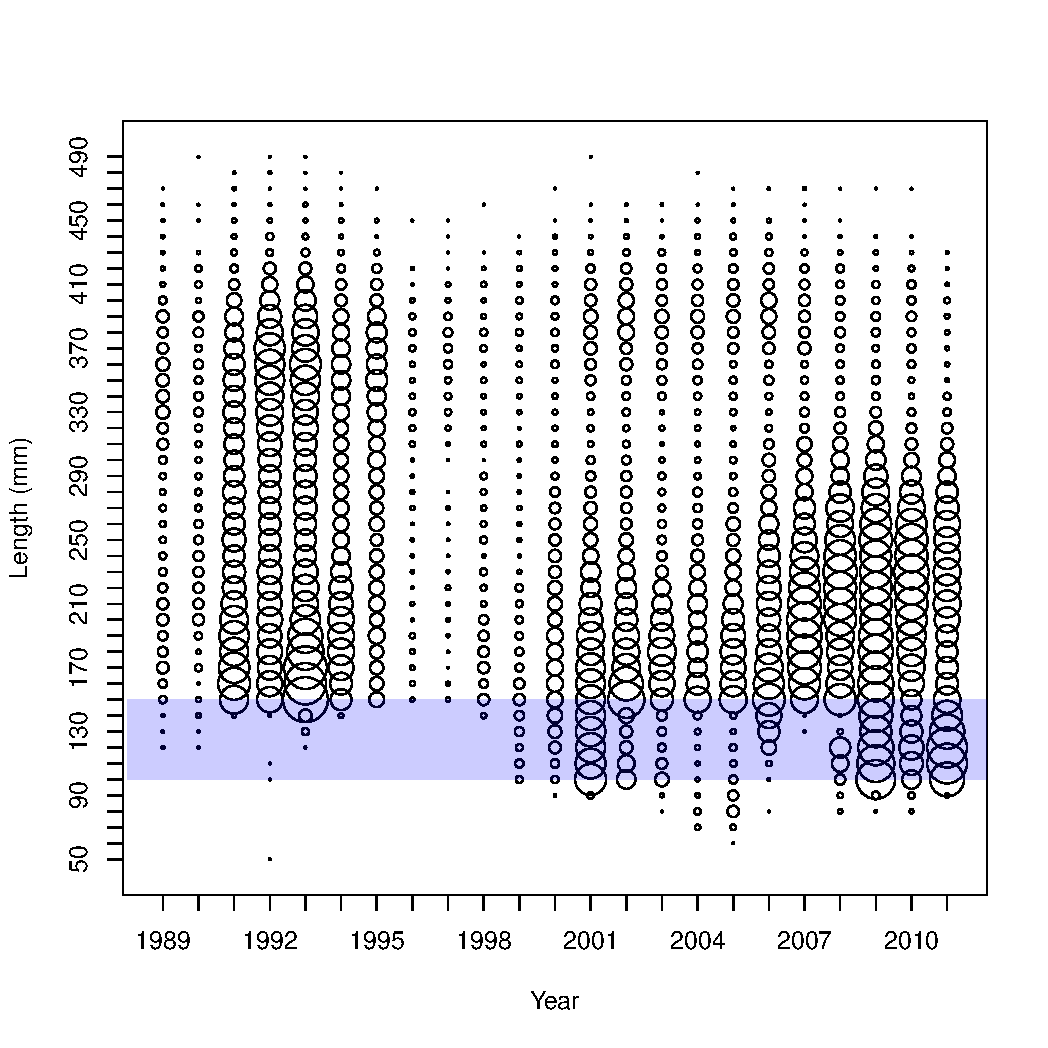
\includegraphics[width=6.5in]{../FIGS/LSMR/fig:CaptureLFbubbles.pdf}
	\caption{Length frequency by year for all gear types. Area of circle is proportional to abundance of measured fish, shaded region represents the 100-150 mm size interval.}
	\label{fig:FIGS_LSMR_fig:CaptureLFbubbles}
\end{figure}

The majority of humpback chub are sampled through the months of April-June and in the fall in September-October (Table \ref{table:Captures}).  Also, the majority of humpback chub are sampled using primarily hoop nets and less so with tramel nets (Table \ref{table:Gear}).  In an attempt to reduce the level of confounding associated with the many different gear types that sample humpback chub, the length composition data was partitioned into two general gear types: (1) hoop nets, ranging in diameter from 2' to 4' with and without bait, and (2) tramel nets of various lengths.  Catch-at-length data by year for hoop nets is shown in Figure \ref{fig:FIGS_LSMR_fig:MarksAtLengthHOOP}.  In the initial years (1989-1990), there are very few recaptures as the marked proportion in the population was relatively low; in subsequent years the marked proportion recaptured increases.  Sampling effort was very low in 1996-1998, resulting in very few fish captured. As time progresses the number of newly marked large fish (greater than 300mm) decreases as most of these individuals were marked in previous years.

\begin{figure}[htbp]
	\centering
		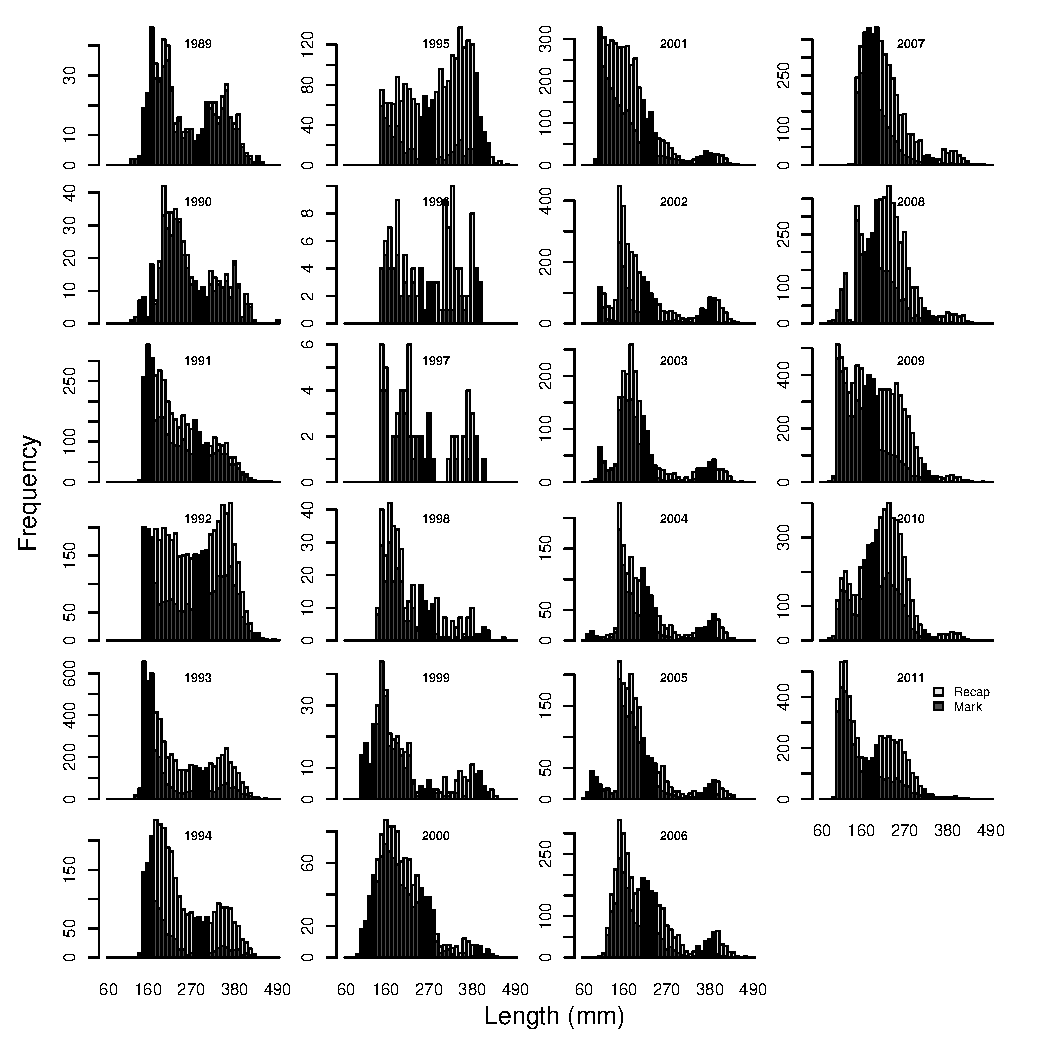
\includegraphics[width=6.5in]{../FIGS/LSMR/fig:MarksAtLengthHOOP.pdf}
	\caption{Annual initial-capture and mark (dark bars) and recapture (light bars) history of HBC using hoop nets (all sizes \& bait) in the LCR and COR reaches from 1989 to 2011.}
	\label{fig:FIGS_LSMR_fig:MarksAtLengthHOOP}
\end{figure}

Far fewer humpback chub have been captured in tramel net gear in comparison to hoopnets, and this is largely due the less frequent use of tramel nets.  Similar patterns in the mark rates were also obtained with the tramel net catch (Figure \ref{fig:FIGS_LSMR_fig:MarksAtLengthGILL}).  Since 1994, tramel net effort for catching humpback chub has been greatly reduced (Table \ref{table:Effort}).  In 2001, the number of tramel net sets with non-zero catches of humpback chub increased to 167 sets, with a very large recapture proportion for fish greater than 300mm.  This observation is also consistent with the large recapture proportion of $>$300mm fish in the hoop net sets in 2001.  Similarly, in 2007, 225 humpback chub were caught in 144 non-zero tramel net sets and the majority of these fish were less than 250mm and never previously marked (Figure \ref{fig:FIGS_LSMR_fig:MarksAtLengthGILL}). Again, this is also consistent with the large number of unmarked fish less than 250mm captured in hoop nets in 2007.

\begin{figure}[htbp]
	\centering
		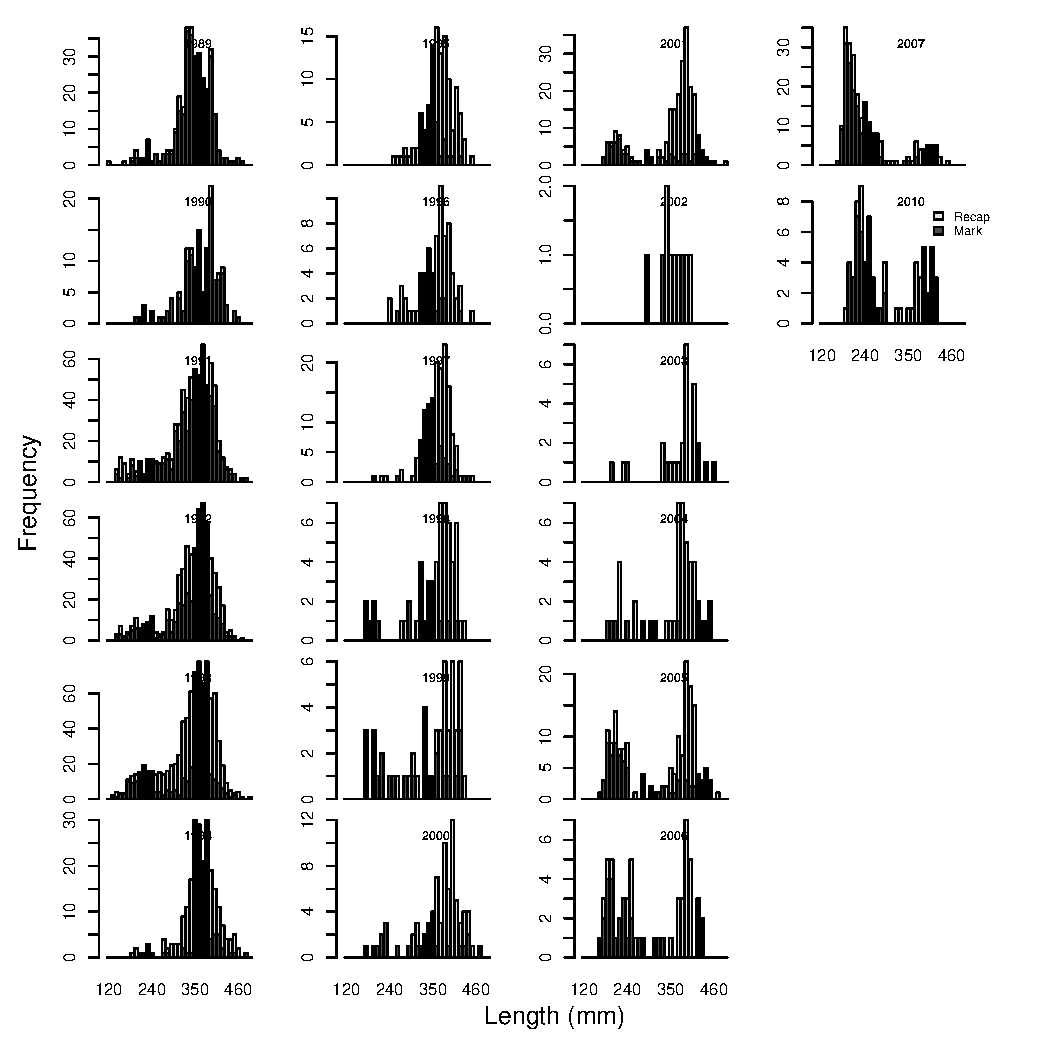
\includegraphics[width=6.5in]{../FIGS/LSMR/fig:MarksAtLengthGILL.pdf}
	\caption{Annual capture and recapture history of HBC using tramel nets of all sizes in the LCR and COR reaches from 1989 to 2011.}
	\label{fig:FIGS_LSMR_fig:MarksAtLengthGILL}
\end{figure}

% latex.default(tx, file = fn, rowname = NULL, caption = cap, size = "footnotesize",      cgroup = cgrp, n.cgroup = ncgrp, label = "table:Captures") 
%
\begin{table}[!tbp]
 \footnotesize
 \caption{Number of fish measured by year and month, sampled by all gears
                  in all reaches of both the LRC and COR.\label{table:Captures}} 
 \begin{center}
 \begin{tabular}{lcrrrrrrrrrrrrr}\hline\hline
\multicolumn{1}{c}{\bfseries }&
\multicolumn{1}{c}{\bfseries }&
\multicolumn{13}{c}{\bfseries MONTH}
\tabularnewline \cline{1-15}
\multicolumn{1}{c}{YEAR}&\multicolumn{1}{c}{}&\multicolumn{1}{c}{1}&\multicolumn{1}{c}{2}&\multicolumn{1}{c}{3}&\multicolumn{1}{c}{4}&\multicolumn{1}{c}{5}&\multicolumn{1}{c}{6}&\multicolumn{1}{c}{7}&\multicolumn{1}{c}{8}&\multicolumn{1}{c}{9}&\multicolumn{1}{c}{10}&\multicolumn{1}{c}{11}&\multicolumn{1}{c}{12}&\multicolumn{1}{c}{(all)}\tabularnewline
\hline
1989&&$  0$&$   0$&$   0$&$    0$&$  887$&$    0$&$   0$&$   0$&$   0$&$   0$&$   0$&$  0$&$  887$\tabularnewline
1990&&$  0$&$   0$&$   0$&$  408$&$  125$&$    0$&$   0$&$   0$&$   0$&$  43$&$  42$&$  0$&$  618$\tabularnewline
1991&&$ 79$&$   3$&$ 135$&$    9$&$  285$&$  394$&$1624$&$1054$&$ 536$&$ 291$&$ 200$&$176$&$ 4786$\tabularnewline
1992&&$168$&$ 340$&$ 781$&$ 1293$&$  493$&$ 1181$&$ 369$&$ 145$&$ 144$&$ 290$&$ 267$&$  0$&$ 5471$\tabularnewline
1993&&$117$&$ 153$&$1132$&$  759$&$ 1359$&$  822$&$ 953$&$1093$&$ 270$&$ 228$&$ 250$&$239$&$ 7375$\tabularnewline
1994&&$154$&$ 201$&$ 296$&$  658$&$  707$&$  410$&$ 198$&$ 154$&$ 152$&$ 129$&$ 128$&$ 55$&$ 3242$\tabularnewline
1995&&$226$&$ 231$&$ 383$&$  915$&$  476$&$   83$&$   0$&$   0$&$   2$&$   0$&$   0$&$  0$&$ 2316$\tabularnewline
1996&&$  0$&$   2$&$  20$&$   96$&$   47$&$    6$&$   0$&$   0$&$  27$&$   0$&$   0$&$  0$&$  198$\tabularnewline
1997&&$  0$&$   0$&$   7$&$   42$&$  114$&$   18$&$   0$&$   0$&$  32$&$   0$&$   0$&$  0$&$  213$\tabularnewline
1998&&$  0$&$   0$&$   1$&$  234$&$   47$&$   36$&$  39$&$  65$&$   5$&$  18$&$   0$&$  0$&$  445$\tabularnewline
1999&&$ 20$&$   0$&$   0$&$  210$&$   52$&$   18$&$   0$&$   0$&$  62$&$  56$&$  53$&$  0$&$  471$\tabularnewline
2000&&$ 20$&$   0$&$   0$&$  418$&$   21$&$  271$&$   2$&$  44$&$  20$&$ 333$&$ 151$&$ 13$&$ 1293$\tabularnewline
2001&&$  0$&$   0$&$   1$&$   37$&$  491$&$ 1347$&$   9$&$ 163$&$  85$&$1180$&$ 929$&$  0$&$ 4242$\tabularnewline
2002&&$  0$&$   4$&$   0$&$  980$&$ 1066$&$    0$&$  20$&$   0$&$ 789$&$ 502$&$   0$&$  0$&$ 3361$\tabularnewline
2003&&$ 16$&$  16$&$  48$&$  599$&$  434$&$    0$&$  55$&$  13$&$ 293$&$ 694$&$  21$&$  0$&$ 2189$\tabularnewline
2004&&$ 18$&$  25$&$  51$&$  760$&$  353$&$   23$&$  27$&$  15$&$ 166$&$ 542$&$  32$&$  0$&$ 2012$\tabularnewline
2005&&$ 23$&$  12$&$  44$&$  515$&$  207$&$  285$&$  93$&$  19$&$ 799$&$ 476$&$   0$&$  0$&$ 2473$\tabularnewline
2006&&$ 24$&$  35$&$ 160$&$ 1098$&$  921$&$  679$&$ 179$&$  56$&$ 270$&$ 317$&$   0$&$  0$&$ 3739$\tabularnewline
2007&&$  0$&$   0$&$   2$&$  937$&$ 1545$&$  900$&$  10$&$   0$&$ 805$&$ 569$&$   0$&$  0$&$ 4768$\tabularnewline
2008&&$  0$&$   5$&$   3$&$ 1265$&$ 1735$&$  528$&$1020$&$ 195$&$ 718$&$ 928$&$   0$&$  0$&$ 6397$\tabularnewline
2009&&$  0$&$   0$&$   6$&$ 1225$&$ 4180$&$ 2267$&$ 551$&$ 168$&$ 895$&$1323$&$ 443$&$245$&$11303$\tabularnewline
2010&&$  0$&$   0$&$   2$&$    0$&$ 1466$&$ 2882$&$ 523$&$  14$&$1043$&$ 708$&$   0$&$  0$&$ 6638$\tabularnewline
2011&&$  0$&$   0$&$   0$&$    0$&$ 2796$&$ 2537$&$ 127$&$ 128$&$ 544$&$1042$&$  63$&$ 49$&$ 7286$\tabularnewline
2012&&$ 28$&$  61$&$   0$&$    0$&$    0$&$    0$&$   0$&$   0$&$   0$&$   0$&$   0$&$  0$&$   89$\tabularnewline
(all)&&$893$&$1088$&$3072$&$12458$&$19807$&$14687$&$5799$&$3326$&$7657$&$9669$&$2579$&$777$&$81812$\tabularnewline
\hline
\end{tabular}

\end{center}

\end{table}


% latex.default(tx, file = fn, rowname = NULL, caption = cap, size = "footnotesize",      cgroup = cgrp, n.cgroup = ncgrp, label = "table:Gear") 
%
\begin{table}[!tbp]
 \footnotesize
 \caption{Number of fish captured by gear type listed in the GCMRC database
                  for each year.\label{table:Gear}} 
 \begin{center}
 \begin{tabular}{lcrrrrrrrrrr}\hline\hline
\multicolumn{1}{c}{\bfseries }&
\multicolumn{1}{c}{\bfseries }&
\multicolumn{10}{c}{\bfseries YEAR}
\tabularnewline \cline{1-12}
\multicolumn{1}{c}{YEAR}&\multicolumn{1}{c}{}&\multicolumn{1}{c}{ANGL}&\multicolumn{1}{c}{DIP}&\multicolumn{1}{c}{ELEC}&\multicolumn{1}{c}{GILL}&\multicolumn{1}{c}{HOOP}&\multicolumn{1}{c}{PA}&\multicolumn{1}{c}{SEINE}&\multicolumn{1}{c}{TRAP}&\multicolumn{1}{c}{(all)}&\multicolumn{1}{c}{NA}\tabularnewline
\hline
1989&&$ 6$&$0$&$  0$&$ 321$&$  560$&$   0$&$  0$&$ 0$&$  887$&$ 0$\tabularnewline
1990&&$ 2$&$0$&$  3$&$ 140$&$  473$&$   0$&$  0$&$ 0$&$  618$&$ 0$\tabularnewline
1991&&$ 4$&$0$&$ 44$&$ 711$&$ 3978$&$   0$&$ 11$&$ 1$&$ 4786$&$37$\tabularnewline
1992&&$ 3$&$0$&$ 68$&$ 636$&$ 4740$&$   0$&$ 24$&$ 0$&$ 5471$&$ 0$\tabularnewline
1993&&$ 2$&$0$&$ 80$&$ 876$&$ 6313$&$   0$&$102$&$ 1$&$ 7375$&$ 1$\tabularnewline
1994&&$ 1$&$0$&$  1$&$ 239$&$ 2997$&$   0$&$  2$&$ 1$&$ 3242$&$ 1$\tabularnewline
1995&&$ 1$&$0$&$  7$&$ 118$&$ 2190$&$   0$&$  0$&$ 0$&$ 2316$&$ 0$\tabularnewline
1996&&$ 0$&$0$&$  4$&$  72$&$  113$&$   0$&$  9$&$ 0$&$  198$&$ 0$\tabularnewline
1997&&$ 0$&$0$&$  2$&$ 153$&$   58$&$   0$&$  0$&$ 0$&$  213$&$ 0$\tabularnewline
1998&&$ 0$&$0$&$  5$&$  58$&$  377$&$   0$&$  4$&$ 1$&$  445$&$ 0$\tabularnewline
1999&&$ 0$&$0$&$ 17$&$  54$&$  392$&$   0$&$  1$&$ 7$&$  471$&$ 0$\tabularnewline
2000&&$ 0$&$0$&$  6$&$  81$&$ 1150$&$   0$&$ 55$&$ 1$&$ 1293$&$ 0$\tabularnewline
2001&&$ 5$&$0$&$  1$&$ 233$&$ 4003$&$   0$&$  0$&$ 0$&$ 4242$&$ 0$\tabularnewline
2002&&$ 0$&$0$&$  5$&$  10$&$ 3346$&$   0$&$  0$&$ 0$&$ 3361$&$ 0$\tabularnewline
2003&&$ 0$&$1$&$102$&$  27$&$ 2058$&$   0$&$  1$&$ 0$&$ 2189$&$ 0$\tabularnewline
2004&&$ 2$&$0$&$108$&$  49$&$ 1621$&$ 226$&$  0$&$ 0$&$ 2012$&$ 6$\tabularnewline
2005&&$ 0$&$0$&$228$&$ 174$&$ 1919$&$ 152$&$  0$&$ 0$&$ 2473$&$ 0$\tabularnewline
2006&&$ 0$&$0$&$138$&$  58$&$ 3442$&$ 100$&$  1$&$ 0$&$ 3739$&$ 0$\tabularnewline
2007&&$ 0$&$0$&$  9$&$ 225$&$ 4352$&$ 181$&$  1$&$ 0$&$ 4768$&$ 0$\tabularnewline
2008&&$ 3$&$0$&$  8$&$   0$&$ 4838$&$1527$&$ 21$&$ 0$&$ 6397$&$ 0$\tabularnewline
2009&&$ 0$&$0$&$  6$&$   0$&$ 7706$&$3589$&$  0$&$ 2$&$11303$&$ 0$\tabularnewline
2010&&$ 3$&$0$&$  0$&$  71$&$ 5294$&$1269$&$  0$&$ 0$&$ 6638$&$ 1$\tabularnewline
2011&&$ 0$&$0$&$  0$&$   0$&$ 5376$&$1910$&$  0$&$ 0$&$ 7286$&$ 0$\tabularnewline
2012&&$ 0$&$0$&$  0$&$   0$&$    0$&$  89$&$  0$&$ 0$&$   89$&$ 0$\tabularnewline
(all)&&$32$&$1$&$842$&$4306$&$67296$&$9043$&$232$&$14$&$81812$&$46$\tabularnewline
\hline
\end{tabular}

\end{center}

\end{table}


% subsection length_composition (end)


%!TEX root = /Users/stevenmartell/Documents/CONSULTING/HumpbackChub/HBC_2011_Assessment/WRITEUP/HBCmain.tex


\subsection{Annual growth rates from capture-recapture information} % (fold)
\label{sub:annual_growth_rates_from_capture_recapture_information}

Parameters for the von Bertalanffy growth model were estimated from the annual growth increment data, where the data were restricted to measured individuals recaptured in the subsequent year (Figure \ref{fig:FIGS_LSMR_fig:AnnualGrowthIncrements}).  The fitted growth model assumed a measurement error with a standard deviation equal to 9.14 mm.  This measurement error was based on the standard deviation in total length of individuals captured multiple times within a 20-day period (roughly the duration of a sampling trip).  Quantile regressions on the raw annual growth increment data (Figure \ref{fig:FIGS_LSMR_fig:AnnualGrowthIncrements}) indicate a steeper, more negative, slope in recent years.  Or in other words, annual growth rates have been increasing in recent years.



\begin{figure}[htbp]
	\centering
		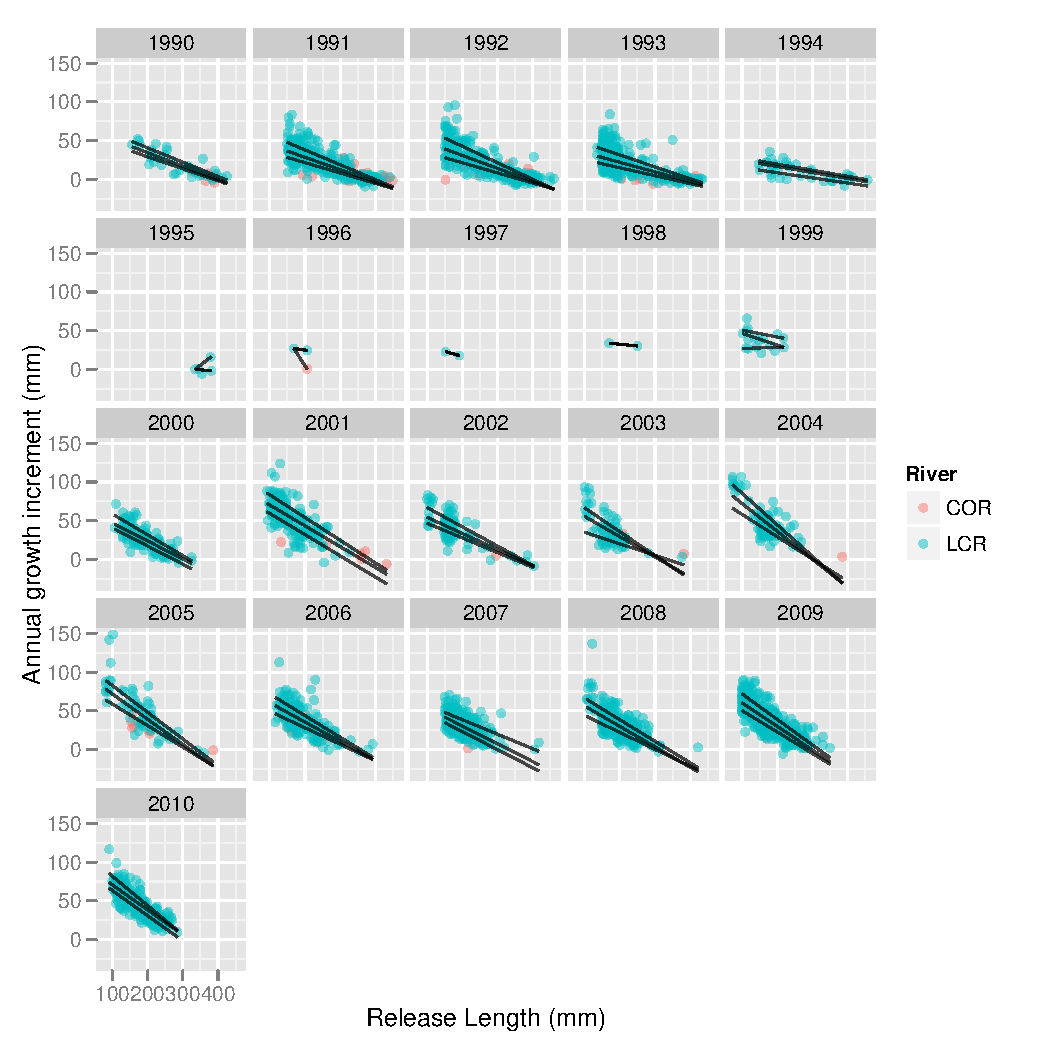
\includegraphics[width=6.5in]{../FIGS/LSMR/fig:GrowthIncrements.pdf}
	\caption{Growth increments by tag year for individually tagged humpback chub that have been at large for at least 1 year.   Recapture events could have occurred in either river. Fitted lines correspond to the 5, 50 and 95 percentiles of the data.}
	\label{fig:FIGS_LSMR_fig:GrowthIncrements}
\end{figure}

\begin{figure}[htbp]
	\centering
		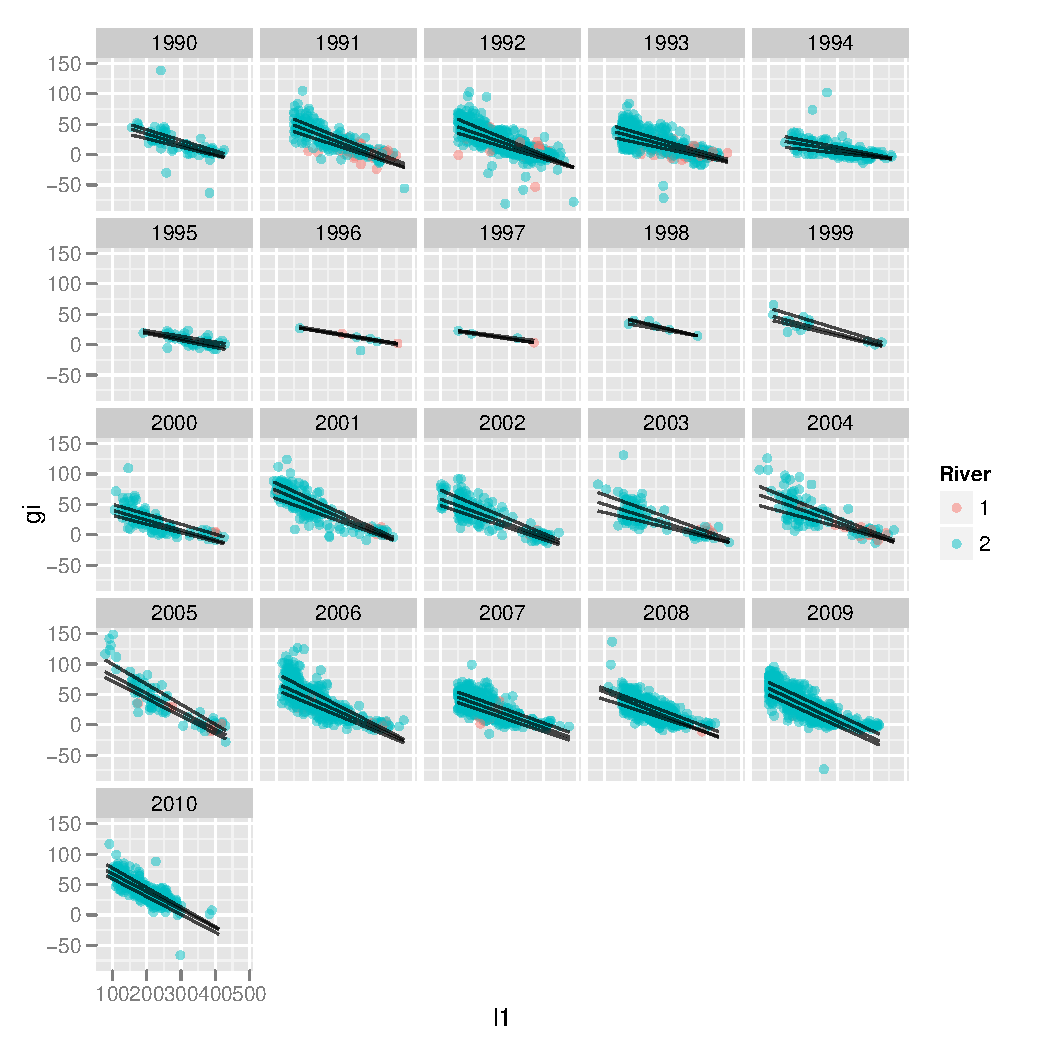
\includegraphics[width=6.5in]{../FIGS/LSMR/fig:AnnualGrowthIncrements.pdf}
	\caption{Annual growth increments of humpback chub of all fish captured and recaptured in the following year. River 2 corresponds to fish tagged in the Little Colorado River, River 1 the Colorado River. Fitted lines correspond to the 5, 50 and 95 percentiles of the data.}
	\label{fig:FIGS_LSMR_fig:AnnualGrowthIncrements}
\end{figure}

Estimated growth parameters based on the annual growth increment data are shown in Figure \ref{fig:FIGS_LSMR_fig:LinfPosteriors}.  Sample sizes between 1995 and 1999 were extremely small and are reflected in the uncertainty in estimates of asymptotic length and $k$.  The median estimate of $l_\infty$ over the entire time series is 373.4 mm with a standard deviation of 28.88 mm.  The overall median estimate of $k$ is 0.246 with a standard deviation of 0.106.  In 2005, the median estimate of $k$ (0.536) was more than twice as large as the overall median estimate owing to the a number of individual fish that were less than 100 mm in 2004 having a growth increment of more than 100 mm in a single year (Figure \ref{fig:FIGS_LSMR_fig:AnnualGrowthIncrements}, year 2005 panel).

\begin{figure}[htbp]
	\centering
		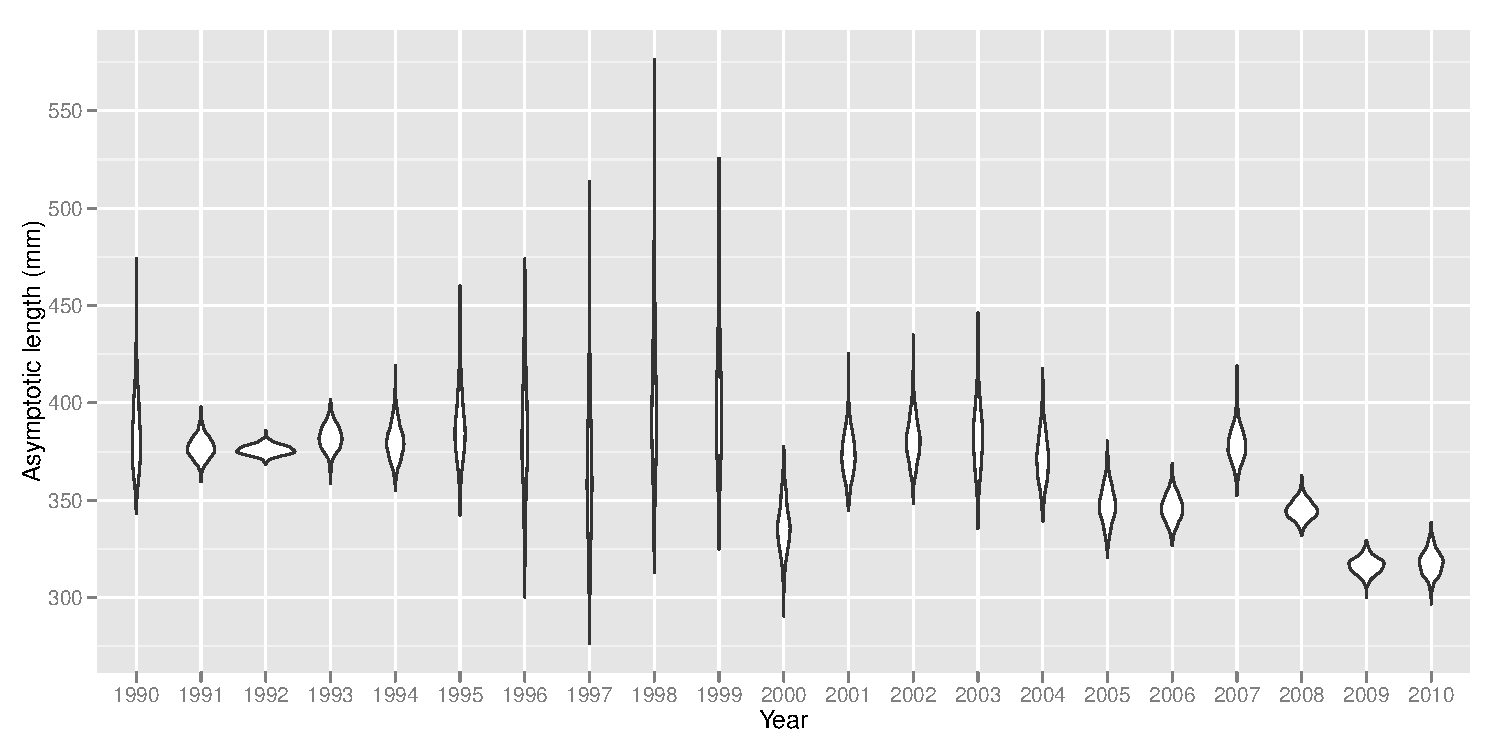
\includegraphics[width=6.5in]{../FIGS/LSMR/fig:LinfPosteriors.pdf}
		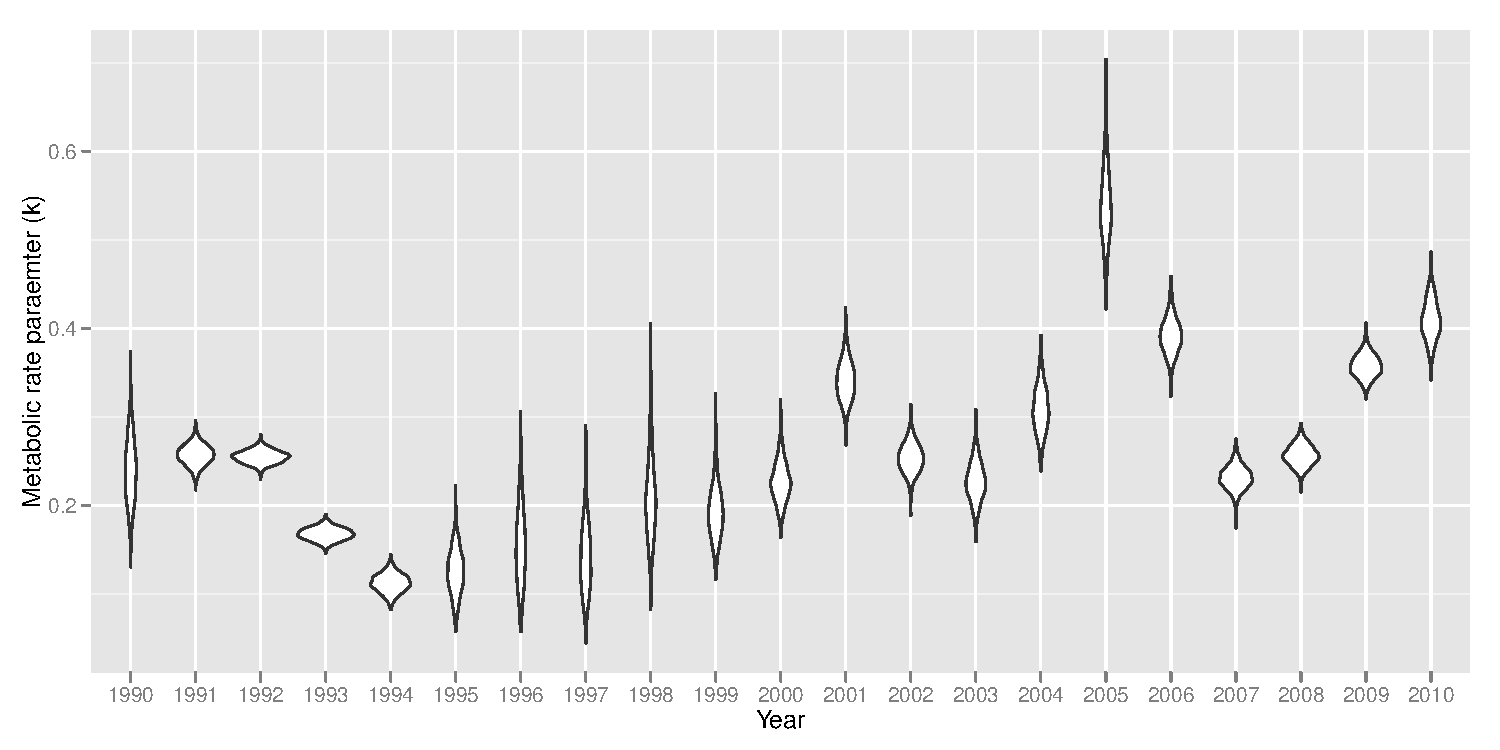
\includegraphics[width=6.5in]{../FIGS/LSMR/fig:kPosteriors.pdf}
	\caption{Violin plots of the marginal posterior distributions for annual estimates of asymptotic length ($l_\infty$, top panel) and the von Bertalanffy metabolic rate parameter ($k$).}
	\label{fig:FIGS_LSMR_fig:LinfPosteriors}
\end{figure}

Estimated growth transition matrices based on the estimated growth parameters from the annual growth increment data are shown in Figure \ref{fig:FIGS_LSMR_fig:TransitionMatrix}. In addition to the transition matrix based, this Figure also has a 1:1 reference line and the corresponding maximum likelihood estimate of $l_\infty$ as a reference to judge differences in the annual length transition matrices.  Starting 2001, growth rates of fish less than 150 mm increased markedly relative to the growth increments observed in the 1990s.  The implications of this increased growth rate in a length-based model would have significant impacts on annual recruitment estimates if growth was assumed to be constant.  The length transition matrices shown in Figure \ref{fig:FIGS_LSMR_fig:TransitionMatrix} provide an alternative input into the length structured mark recapture model (LSMR), where length-transition matrices are estimated externally.


\begin{figure}[htbp]
	\centering
		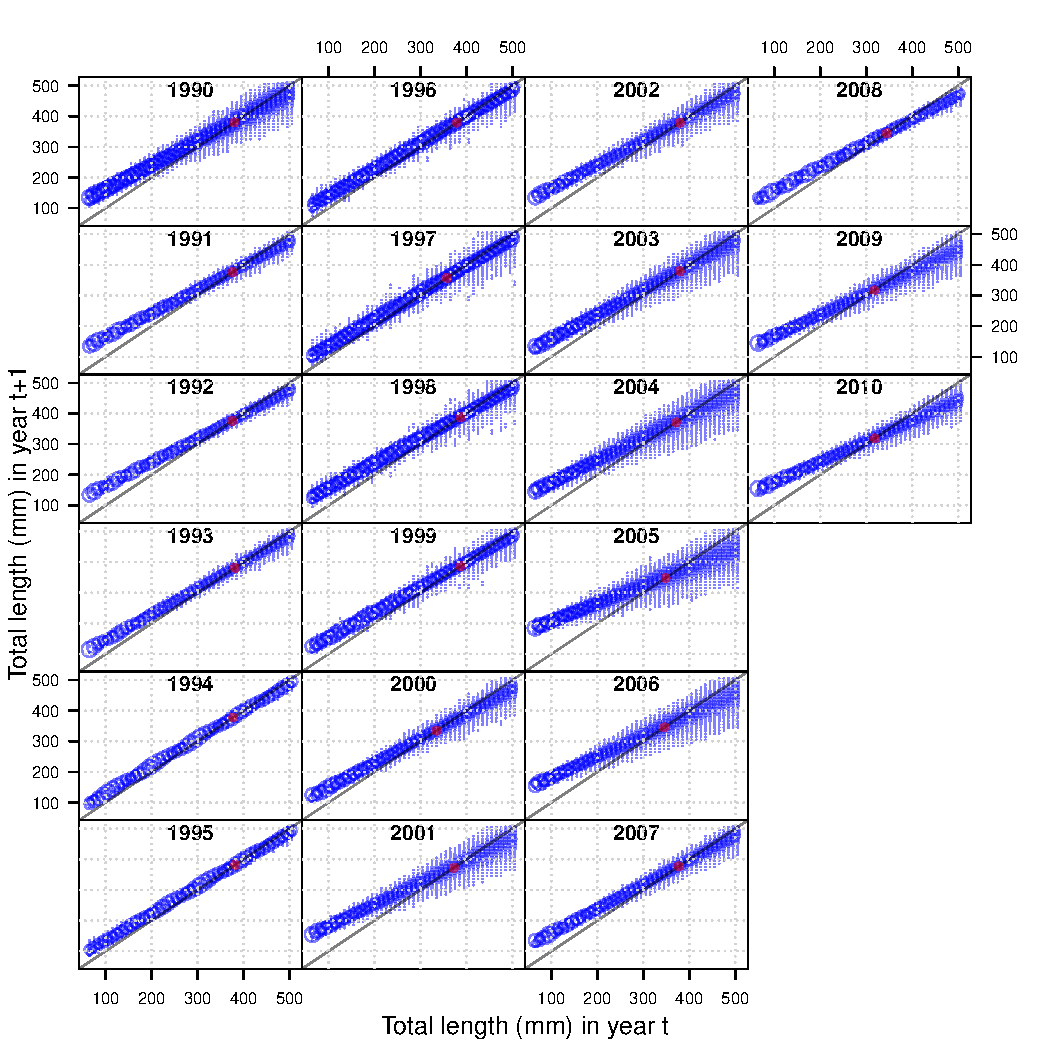
\includegraphics[width=6.5in]{../FIGS/LSMR/fig:TransitionMatrix.pdf}
	\caption{Annual length transition matrixes based on the annual growth increment data.  The area of each bubble is proportional to the transition probability from year $t$ to year $t+1$, the diagonal black line is the 1:1 slope, and the red circle corresponds to the maximum likelihood estimate of $l_\infty$.  Each matrix is based on parametric uncertainty in the estimated von Bertalanffy growth parameters as well as measurement errors. }
	\label{fig:FIGS_LSMR_fig:TransitionMatrix}
\end{figure}


% subsection annual_growth_rates_from_capture_recapture_information (end)

% section results (end)

\bibliographystyle{apalike} 
\bibliography{$HOME/Documents/ARTICLES/Articles-1}

\appendix 
%!TEX root = /Users/stevenmartell/Documents/CONSULTING/HumpbackChub/HBC_2011_Assessment/WRITEUP/HBCmain.tex

\section{Work plan}
The following outlines a work plan for the assessment of abundance for humpback chub. The objective is to develop a much more flexible length-based model that can be used to explore alternative hypotheses about natural mortality rates, cumulative effects of release mortality for intensive sampling periods, and to potentially integrate other sources of environmental variations such as the effects of turbidity on capture probability and recruitment variation.

\section*{Analytical approach}
I will develop a statistical catch-at-length model in the AD Model Builder software and additions R-scripts for manipulating data and summarizing model results.  Input data for the model will consist of a matrix of the total catch-at-length in 5 to 10 mm size intervals for all years, a matrix of the number of marks released by size and year, a matrix of the number of marks recaptured by size and year, and a three dimensional array of the number of marks recaptures by size for each tag-cohort released (optional).

Estimated parameter will include: natural mortality rate, growth parameters, a vector of the initial numbers in each length interval, and a vector of age-0 recruits each year.  Propagation of the numbers-at-length to the next time step will be based on a size-transition matrix, which is a function of the growth parameters and variation in growth.  Observation models will include a probability of capturing an animal of a given length each year, the probabilities of capturing a marked and unmarked animal of a given length, and optionally the probability of recapturing a specific tag-cohort of a given length.  These predicted observations will be compared with the empirical data using a negative binomial likelihood function.  The negative binomial model is more suitable here because it can account for over-dispersed data  and accommodate zero observations in cases where there is sparse information.

\section*{Detailed work plan}

\subsection*{Major components of the project}
The following is list of milestones for this project.  Each of these items will be expanded upon in the section on project details.
\begin{enumerate}
	\item Data acquisition and processing.
	\item Development of an operating model for simulating data with known parameter values.
	\item Development of a length-based assessment model to be fitted to data on capture and recapture information by length interval.
	\item Simulation testing; exploring the precision and bias of the assessment model in jointly estimating recruitment, size-specific capture probability, and growth and natural mortality using simulated data sets.
	\item Application of the length-based model to the HBC data.
	\item Quantifying uncertainty in model parameters and estimates of recruits using Markov Chain Monte Carlo methods to integrate the joint posterior distribution.
	\item Report \& presentation to the Technical Working Group.
\end{enumerate}

\subsection*{Project details}
\begin{description}
	\item[Data acuisition \& processing] The necessary data required to conduct the analysis will require information from the following fields in the GCMRC database: FISHNO, TRIP\_ID, DATES, RM, RIV, TL, TAGNO. The following SQL statement was used in a previous study to extract the necessary information. Note that the following code has been modified to obtain all fish lengths, not just those greater than 150 mm.
	\begin{verbatim}
		--****
		--All
		--****

		CREATE OR REPLACE VIEW FISH.V_ASMR_2009_ALL
		(
		    FISHNO,
		    TRIP_ID,
		    DATES,
		    RM,
		    RIV,
		    TL,
		    TAGNO
		)
		AS
		SELECT "CAPTURE_ID" fishno, "TRIP_ID" trip_id, "START_DATE" dates,"START_RM" rm,"RIVER_CODE" riv, "TOTAL_LENGTH" tl,"TH_ENCOUNTER_RANKING" tagno
		      FROM FISH.CAPTURE_HISTORY_20091211_0832
		     WHERE SPECIES_CODE = 'HBC'
		     AND (
		       (RIVER_CODE = 'COR' AND START_RM >= 57 AND START_RM <= 68.5)
		       OR RIVER_CODE = 'LCR'
		       )
		     AND START_DATE >= TO_DATE('04/01/1989', 'MM/DD/YYYY')
		     AND TOTAL_LENGTH >= 00
		
	\end{verbatim} 
	
	An R-script will be developed for post processing of the data to assign the length capture and recapture information into discrete length intervals for assembling input data into the assessment model.
	
	\item[Operating model] An individual based model will be developed to generate simulated data sets with known natural mortality rates, recruitment vectors, growth rates and capture probabilities.  The pseudo code for the operating model is as follows:
	\begin{enumerate}
		\item Specify a vector of absolute recruitment from 1950-2011.
		\item For each individual recruit in each year apply the following procedure:
		\begin{enumerate}
			\item boolean trail for survival, if the animal survives then go to (b) else, individual died and restart at step 2.
			\item boolean trail for capture:
			\begin{enumerate}
				\item Captured: obtain length of fish, if greater than 150mm then tag and release fish, go.
				\item Recaptured: obtain length of fish, goto step (a).
				\item Not captured: goto step (a).
			\end{enumerate}
		\end{enumerate}
		\item Store information about individual capture history and length into simulated database.
	\end{enumerate}
	The above algorithm is intended to generate the exact data that is currently collected in the HBC monitoring program. Specific details about factors that affect capture probability and survival would be incorporated into the boolean probabilities defined in 2a and 2b.
	
	\item[Length-based assessment model] A statistical length-based assessment model is similar in nature to a statistical catch-age model in that numbers-at-age, or in this case, numbers-at-length are propagated forward in time.  The previous Age-Structured Mark-Recapture Model (ASMR) was dependent on catch-age information; age data for HBC were inferred from an analytical age-length key (i.e., based on inferences about growth, not empirical age-length data).  Estimates of uncertainty were overly precise due to the pre-processing of the data to be used with ASMR. The length-based model makes no such inferences about the age of individual fish and is based strictly on the length observation data.  
	
	In a length based model, individuals in a given length interval are propagated in time by redistributing these individuals into new length bins based on a length transition probability (Fig \ref{fig:lengthTransition}).  The length transition probability is a function of growth and the time interval between sampling events.  The graphical example in Fig \ref{fig:lengthTransition} does not account for mortality over time, its only meant to show the transition of individuals from one length bin to subsequent length bins.
	\begin{figure}[htbp]
		\centering
			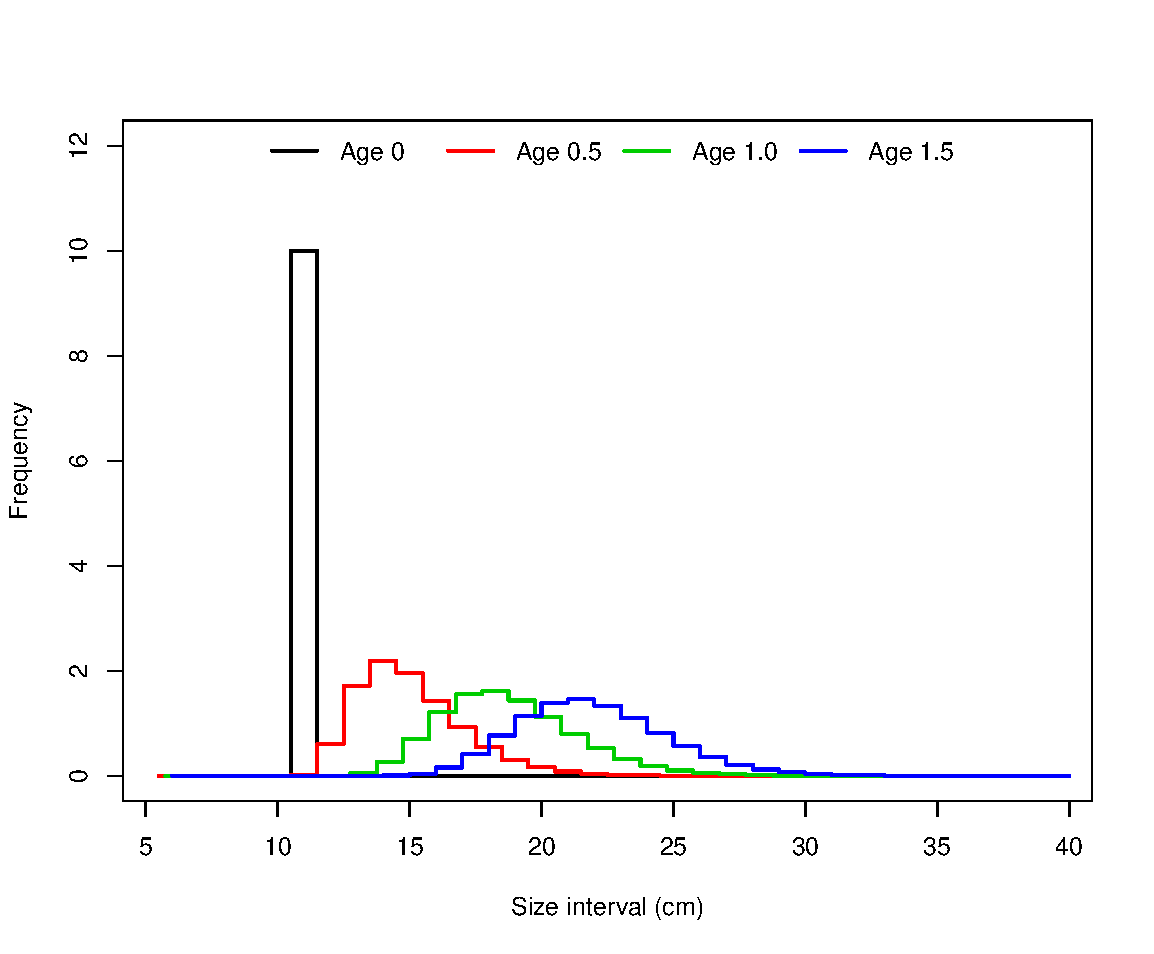
\includegraphics[scale=0.65]{../FIGS/fig:lengthTransition}
		\caption{A graphical example of a length-based transition. Starting with 10 age-0 individuals, these 10 would then be distributed to the age-0.5 distribution distribution.  The age-0.5 distribution then transitions to the age-1.0 distribution and so on.}
		\label{fig:lengthTransition}
	\end{figure}
	
	\item[Simulation testing] The purpose of simulation testing is to (i) demonstrate that the model is able to estimate the model parameters given perfect information and satisfying all of the model assumptions, (ii) examine precision and bias in parameter estimates when faced with observation, process, and structural errors, and lastly (iii) to examine the estimability, bias, and precision of model parameters when underlying structural assumptions are not met.  Simulation testing will be conducted to examine the ability to jointly estimate recruitment, capture probability, growth and natural mortality in a reliable and unbiased manner.
	
	\item[Application to the HBC data] The length-based assessment model will then be applied to the length-based capture and recapture data for the humpback chub monitoring program.  Model outputs will include estimates of recruits (and associated uncertainty), estimated model parameters (and uncertainty).  It is  anticipated that more reliable estimates of recruits will be available with the length based model because the model is not limited to length information that is greater than 150mm, as is the case in the ASMR model.
	
	\item[Quantifying uncertainty] Estimates of uncertainty will jointly consider uncertainty in the mark-recapture data, growth and mortality.  To do so the joint posterior distribution of the data will be constructed numerically using a Markov Chain Monte Carlo procedure (using the Metropolis Hastings algorithm implemented in AD Model Builder).  Uncertainty in model parameters as well as outputs will be cast in the form of marginal posterior densities.
	
	\item[Report and presentation] This is original research and the methods outlined for a length-based model that incorporates growth increment data from a mark recapture program has not been previously published to my knowledge. Ideally these results will be disseminated in the primary literature, but will also be presented to the Technical Working Group and be available as a technical report (e.g., USGS Open File Report).  Also source code, scripts, and documentation will be hosted on an open source repository with version control.  The intention here is to create a repository for continued development of the software and to document the historical changes over time.
\end{description}
 
%!TEX root = /Users/stevenmartell/Documents/CONSULTING/HumpbackChub/HBC_2011_Assessment/WRITEUP/HBCmain.tex
\section{Individual based model for simulating the dynamics and sampling of humpback chub in the Grand Canyon}

\subsection{Introduction}
The following is a detailed description of the simulation model that was used for simulating the population dynamics and data collection programs for humpback chub in the Grand canyon. We first describe in detail the life-history trajectory of an individual fish: the survival probability, growth, and capture history and provide the documented code to implement this process. I then describe the data structures that resemble a databased of individual capture histories for both tagged and untagged fish.   The individual based model (IBM) is then used to estimate the fate and capture histories of a known number of recruits starting life at a 40mm length interval.

The simulation model was constructed using R \citep{R-Development-Core-Team:2009fk}.  The algorithm populates three matrixes that contain the total number of fish captured in year $t$ at length interval $x$, the total number of newly marked fish, and a matrix of the total number of recaptured individuals.  At each time step the fish is alive, information on length and age is stored along with information on capture history, the tag number if the fish was large enough to tag.

\subsection{R-code}
\lstinputlisting[language=R]{../R/HBCsim.R}
%!TEX root = /Users/stevenmartell/Documents/CONSULTING/HumpbackChub/HBC_2011_Assessment/WRITEUP/HBCmain.tex
\section{Processing mark-recapture by length information} % (fold)
\label{sec:processing_mark_recapture_by_length_information}

The following description details how the raw data from the GCMRC database was used to construct the tables of data used in this assessment. The raw data obtained from Glenn Bennet (\texttt{gbennet@usgs.gov}) contained the following fields:
\begin{scriptsize}
\begin{verbatim}
CAPTURE_ID SPECIES_CODE    TRIP_ID     START_DATETIME START_RM RIVER_CODE TOTAL_LENGTH TH_ENCOUNTER_RANKING GEAR_CODE
      1496          HBC LC20000417 4/17/2000 17:15:00       NA        LCR          380                20397        HS
        48          HBC LC20000417 4/18/2000 16:10:00       NA        LCR          285                49293        HS
        49          HBC LC20000417 4/18/2000 16:10:00       NA        LCR          219                49220        HS
       100          HBC LC20000417  4/18/2000 8:06:00       NA        LCR          170                49255        HS
       156          HBC LC20000417 4/17/2000 18:20:00       NA        LCR          325                49238        HS
       241          HBC LC20000417 4/18/2000 17:15:00       NA        LCR          214                49309        HS
\end{verbatim}
\end{scriptsize}
The \verb"TH_ENCOUNTER_RANKING" field is a unique number for each individual marked fish and occurs in the database one or more times depending on the number of recapture events for that individual, this is also referred to as the \verb"TAGNO".  At the time of writing this report, there were a total of 81,812 records in the database for humpback chub, of which 35,696 are unique individuals (some of which may occur in the database only once).  These data were first imported into R \citep{R-Development-Core-Team:2009fk}, the year and month was then extracted from the \verb"START_DATETIME" field and appended to the data frame.  Next the total length of measured humpback chub were assigned to corresponding 10mm size intervals ranging from 50mm to 600mm.  Note that the R-code for manipulating the database can be found in subsection \ref{sub:r_code_for_database_manipulation}.

There are 110 unique \verb"GEAR_CODE"s in the database; these gear codes were classified into 12 gear groups, of which tramel nets (GILL)  and hoop nets (HOOP) were used to reconstruct the marks and recaptures at length.

The last step in constructing the data frame (see the function \verb"get.DF") was to assign initial marks and recapture event to each of the records.  To do so, the data frame was ordered by date and tag number in ascending order and all duplicate occurrences of \verb"TAGNO" were assigned a boolean TRUE value.  The additional columns added to the data frame was necessary to extract the total number of fish caught by month in each year (Table \ref{table:Captures}), and the total number fish captured each year by specific gear types (Table \ref{table:Gear}).

Key input data to the LSMR assessment model is the number of marked fish released (by size class) and the number of recaptured fish (by size class) in subsequent sampling events by specific gear types.  To construct these data, an R-function (\verb"tableMarks") was developed to construct Tables \ref{sidewaystable:Mark_HOOP}--\ref{sidewaystable:Recapture_GILL}.  I only consider marks and recaptures from the hoop nets and gillnet (tramel nets) sampling gears in this analysis, as these two gear types were responsible for sampling the majority of humpback chub in the system.


% latex.default(LI, file = fn, caption = cap, size = "tiny", cgroup = cgrp,      n.cgroup = ncgrp, lable = "sidewaystable:Lf") 
%
\begin{sidewaystable}[!tbp]
\tiny
\caption{Number of fish captured by length by all gear types 
                  listed in the GCMRC database for each year.\label{LI}} 
\begin{center}
\begin{tabular}{lrcrrrrrrrrrrrrrrrrrrrrrr}
\hline\hline
\multicolumn{1}{l}{\bfseries LI}&
\multicolumn{1}{c}{\bfseries }&
\multicolumn{1}{c}{\bfseries }&
\multicolumn{22}{c}{\bfseries YEAR}
\tabularnewline
\cline{4-25}
\multicolumn{1}{l}{}&\multicolumn{1}{c}{1989}&\multicolumn{1}{c}{}&\multicolumn{1}{c}{1990}&\multicolumn{1}{c}{1991}&\multicolumn{1}{c}{1992}&\multicolumn{1}{c}{1993}&\multicolumn{1}{c}{1994}&\multicolumn{1}{c}{1995}&\multicolumn{1}{c}{1996}&\multicolumn{1}{c}{1997}&\multicolumn{1}{c}{1998}&\multicolumn{1}{c}{1999}&\multicolumn{1}{c}{2000}&\multicolumn{1}{c}{2001}&\multicolumn{1}{c}{2002}&\multicolumn{1}{c}{2003}&\multicolumn{1}{c}{2004}&\multicolumn{1}{c}{2005}&\multicolumn{1}{c}{2006}&\multicolumn{1}{c}{2007}&\multicolumn{1}{c}{2008}&\multicolumn{1}{c}{2009}&\multicolumn{1}{c}{2010}&\multicolumn{1}{c}{2011}\tabularnewline
\hline
50&$ 0$&&$ 0$&$  0$&$  1$&$  0$&$  0$&$  0$&$ 0$&$ 0$&$ 0$&$ 0$&$ 0$&$  0$&$  0$&$  0$&$  0$&$  0$&$  0$&$  0$&$  0$&$  0$&$  0$&$  0$\tabularnewline
60&$ 0$&&$ 0$&$  0$&$  0$&$  0$&$  0$&$  0$&$ 0$&$ 0$&$ 0$&$ 0$&$ 0$&$  0$&$  0$&$  0$&$  0$&$  1$&$  0$&$  0$&$  0$&$  0$&$  0$&$  0$\tabularnewline
70&$ 0$&&$ 0$&$  0$&$  0$&$  0$&$  0$&$  0$&$ 0$&$ 0$&$ 0$&$ 0$&$ 0$&$  0$&$  0$&$  0$&$ 10$&$ 11$&$  0$&$  0$&$  0$&$  0$&$  0$&$  0$\tabularnewline
80&$ 0$&&$ 0$&$  0$&$  0$&$  0$&$  0$&$  0$&$ 0$&$ 0$&$ 0$&$ 0$&$ 0$&$  0$&$  0$&$  1$&$ 15$&$ 45$&$  1$&$  0$&$  7$&$  2$&$  6$&$  0$\tabularnewline
90&$ 0$&&$ 0$&$  0$&$  0$&$  0$&$  0$&$  0$&$ 0$&$ 0$&$ 0$&$ 0$&$ 2$&$ 14$&$  0$&$  5$&$  7$&$ 35$&$  0$&$  0$&$ 10$&$ 21$&$ 13$&$  6$\tabularnewline
100&$ 0$&&$ 0$&$  0$&$  1$&$  0$&$  0$&$  0$&$ 0$&$ 0$&$ 0$&$17$&$18$&$327$&$118$&$ 65$&$  5$&$ 23$&$  2$&$  0$&$ 37$&$514$&$117$&$393$\tabularnewline
110&$ 0$&&$ 0$&$  0$&$  1$&$  0$&$  0$&$  0$&$ 0$&$ 0$&$ 0$&$24$&$24$&$304$&$ 97$&$ 40$&$  6$&$ 15$&$ 10$&$  0$&$ 95$&$465$&$180$&$538$\tabularnewline
120&$ 3$&&$ 1$&$  0$&$  0$&$  1$&$  0$&$  0$&$ 0$&$ 0$&$ 0$&$17$&$47$&$286$&$ 56$&$ 22$&$  9$&$ 17$&$ 71$&$  0$&$140$&$424$&$201$&$539$\tabularnewline
130&$ 2$&&$ 2$&$  0$&$  0$&$ 18$&$  0$&$  0$&$ 0$&$ 0$&$ 0$&$28$&$57$&$297$&$ 50$&$ 25$&$ 11$&$  9$&$153$&$  2$&$ 10$&$334$&$165$&$403$\tabularnewline
140&$ 3$&&$ 7$&$  5$&$  2$&$ 54$&$  8$&$  0$&$ 0$&$ 0$&$10$&$30$&$71$&$289$&$ 76$&$ 34$&$ 20$&$ 13$&$213$&$  1$&$  3$&$371$&$132$&$304$\tabularnewline
150&$19$&&$ 8$&$268$&$221$&$684$&$147$&$ 76$&$ 6$&$ 6$&$43$&$45$&$83$&$280$&$447$&$166$&$229$&$248$&$345$&$245$&$333$&$436$&$132$&$239$\tabularnewline
160&$24$&&$ 2$&$353$&$215$&$585$&$163$&$ 63$&$ 9$&$ 5$&$26$&$37$&$91$&$281$&$382$&$216$&$162$&$218$&$310$&$333$&$257$&$424$&$213$&$162$\tabularnewline
170&$47$&&$18$&$318$&$194$&$618$&$209$&$ 62$&$ 7$&$ 1$&$44$&$22$&$89$&$283$&$259$&$208$&$116$&$204$&$267$&$371$&$201$&$359$&$235$&$159$\tabularnewline
180&$34$&&$ 7$&$270$&$211$&$450$&$235$&$ 62$&$ 8$&$ 2$&$39$&$23$&$88$&$240$&$233$&$264$&$141$&$215$&$210$&$394$&$238$&$399$&$278$&$148$\tabularnewline
190&$31$&&$19$&$296$&$188$&$400$&$229$&$ 88$&$10$&$ 3$&$35$&$20$&$88$&$259$&$222$&$208$&$106$&$190$&$168$&$401$&$259$&$385$&$283$&$159$\tabularnewline
200&$46$&&$43$&$262$&$213$&$295$&$224$&$ 65$&$ 3$&$ 5$&$30$&$19$&$64$&$190$&$167$&$159$&$102$&$165$&$176$&$415$&$349$&$322$&$325$&$211$\tabularnewline
210&$42$&&$35$&$215$&$193$&$216$&$189$&$ 82$&$ 5$&$ 4$&$11$&$16$&$67$&$164$&$151$&$125$&$122$&$124$&$198$&$374$&$352$&$345$&$362$&$247$\tabularnewline
220&$28$&&$37$&$176$&$188$&$235$&$182$&$ 76$&$ 2$&$ 7$&$13$&$20$&$65$&$118$&$135$&$ 97$&$ 94$&$ 81$&$192$&$328$&$354$&$347$&$390$&$239$\tabularnewline
230&$21$&&$35$&$168$&$201$&$205$&$139$&$ 66$&$ 4$&$ 3$&$17$&$ 6$&$50$&$129$&$ 97$&$ 51$&$ 74$&$ 79$&$171$&$291$&$385$&$346$&$409$&$246$\tabularnewline
240&$17$&&$34$&$152$&$161$&$156$&$105$&$ 61$&$ 4$&$ 2$&$ 4$&$ 3$&$52$&$ 81$&$ 80$&$ 32$&$ 54$&$ 68$&$162$&$258$&$338$&$329$&$361$&$231$\tabularnewline
250&$14$&&$25$&$180$&$156$&$153$&$ 82$&$ 49$&$ 4$&$ 2$&$17$&$ 5$&$44$&$ 65$&$ 62$&$ 25$&$ 40$&$ 50$&$131$&$206$&$299$&$368$&$358$&$221$\tabularnewline
260&$13$&&$23$&$153$&$156$&$154$&$ 74$&$ 71$&$ 2$&$ 2$&$12$&$ 5$&$39$&$ 59$&$ 41$&$ 23$&$ 29$&$ 61$&$122$&$147$&$229$&$324$&$313$&$232$\tabularnewline
270&$15$&&$15$&$144$&$152$&$177$&$ 81$&$ 58$&$ 6$&$ 5$&$10$&$ 6$&$38$&$ 53$&$ 36$&$ 16$&$ 24$&$ 31$&$ 78$&$150$&$257$&$271$&$244$&$183$\tabularnewline
280&$12$&&$15$&$171$&$167$&$177$&$ 70$&$ 67$&$ 5$&$ 1$&$12$&$ 4$&$30$&$ 41$&$ 41$&$ 15$&$ 27$&$ 23$&$ 70$&$ 92$&$155$&$245$&$178$&$154$\tabularnewline
290&$14$&&$14$&$140$&$160$&$170$&$ 72$&$ 74$&$ 4$&$ 0$&$15$&$ 4$&$16$&$ 30$&$ 35$&$ 17$&$ 14$&$ 14$&$ 51$&$ 86$&$101$&$183$&$121$&$102$\tabularnewline
300&$22$&&$12$&$126$&$174$&$155$&$ 64$&$ 98$&$ 3$&$ 1$&$ 1$&$ 4$&$ 9$&$ 22$&$ 26$&$  9$&$ 10$&$ 15$&$ 55$&$ 65$&$101$&$129$&$ 71$&$ 85$\tabularnewline
310&$40$&&$13$&$131$&$191$&$175$&$ 72$&$ 80$&$10$&$ 4$&$ 8$&$ 8$&$11$&$ 11$&$ 16$&$  5$&$  8$&$ 10$&$ 32$&$ 69$&$ 72$&$ 89$&$ 46$&$ 51$\tabularnewline
320&$37$&&$18$&$137$&$223$&$215$&$ 68$&$ 90$&$12$&$ 8$&$ 5$&$ 2$&$ 9$&$ 14$&$ 13$&$  8$&$ 10$&$  6$&$ 15$&$ 26$&$ 42$&$ 65$&$ 32$&$ 38$\tabularnewline
330&$59$&&$27$&$157$&$244$&$207$&$ 89$&$113$&$14$&$14$&$ 7$&$ 6$&$ 8$&$ 10$&$ 19$&$  6$&$ 10$&$ 14$&$ 10$&$ 28$&$ 34$&$ 39$&$ 20$&$ 19$\tabularnewline
340&$54$&&$25$&$147$&$255$&$259$&$109$&$113$&$10$&$15$&$ 7$&$ 7$&$10$&$ 19$&$ 20$&$ 20$&$ 18$&$ 17$&$ 16$&$ 20$&$ 20$&$ 20$&$ 10$&$ 17$\tabularnewline
350&$54$&&$20$&$149$&$287$&$292$&$116$&$151$&$ 8$&$14$&$10$&$10$&$ 8$&$ 34$&$ 27$&$ 27$&$ 23$&$ 18$&$ 28$&$ 18$&$ 18$&$ 22$&$ 11$&$  5$\tabularnewline
360&$59$&&$30$&$151$&$292$&$329$&$116$&$133$&$ 9$&$23$&$ 6$&$10$&$20$&$ 39$&$ 49$&$ 33$&$ 30$&$ 15$&$ 18$&$ 16$&$ 19$&$ 19$&$ 20$&$  6$\tabularnewline
370&$40$&&$17$&$133$&$313$&$242$&$105$&$137$&$13$&$23$&$15$&$ 9$&$14$&$ 53$&$ 44$&$ 35$&$ 34$&$ 37$&$ 45$&$ 50$&$ 20$&$ 15$&$ 24$&$  5$\tabularnewline
380&$36$&&$31$&$108$&$231$&$236$&$ 90$&$135$&$15$&$26$&$18$&$17$&$18$&$ 57$&$ 86$&$ 52$&$ 49$&$ 40$&$ 54$&$ 38$&$ 33$&$ 23$&$ 21$&$  7$\tabularnewline
390&$50$&&$35$&$108$&$181$&$187$&$ 73$&$103$&$12$&$18$&$ 8$&$11$&$15$&$ 64$&$ 84$&$ 60$&$ 58$&$ 57$&$ 76$&$ 43$&$ 25$&$ 26$&$ 31$&$  8$\tabularnewline
400&$21$&&$ 9$&$ 72$&$123$&$145$&$ 46$&$ 52$&$ 7$&$ 8$&$ 6$&$15$&$20$&$ 46$&$ 77$&$ 38$&$ 43$&$ 51$&$ 81$&$ 44$&$ 25$&$ 18$&$ 24$&$ 11$\tabularnewline
410&$ 8$&&$17$&$ 38$&$ 77$&$ 90$&$ 37$&$ 43$&$ 2$&$ 7$&$10$&$ 7$&$ 7$&$ 43$&$ 51$&$ 35$&$ 32$&$ 38$&$ 36$&$ 32$&$ 19$&$ 18$&$ 25$&$  4$\tabularnewline
420&$ 5$&&$15$&$ 21$&$ 49$&$ 49$&$ 22$&$ 28$&$ 3$&$ 1$&$ 4$&$ 8$&$ 8$&$ 24$&$ 36$&$ 25$&$ 20$&$ 25$&$ 36$&$ 23$&$ 22$&$  7$&$ 11$&$  2$\tabularnewline
430&$ 4$&&$ 4$&$ 12$&$ 16$&$ 20$&$ 10$&$ 11$&$ 0$&$ 1$&$ 1$&$ 4$&$ 6$&$  8$&$ 15$&$ 15$&$  7$&$ 15$&$ 17$&$ 12$&$  6$&$  7$&$  4$&$  2$\tabularnewline
440&$ 4$&&$ 0$&$  8$&$ 18$&$ 11$&$  5$&$  2$&$ 0$&$ 1$&$ 0$&$ 1$&$ 5$&$  4$&$  8$&$  4$&$  8$&$ 12$&$ 12$&$  2$&$  3$&$  2$&$  1$&$  0$\tabularnewline
450&$ 3$&&$ 2$&$  7$&$  7$&$  5$&$  7$&$  5$&$ 1$&$ 1$&$ 0$&$ 0$&$ 1$&$  2$&$  3$&$  1$&$  5$&$  5$&$  5$&$  2$&$  1$&$  0$&$  0$&$  0$\tabularnewline
460&$ 2$&&$ 1$&$  3$&$  3$&$  6$&$  2$&$  0$&$ 0$&$ 0$&$ 1$&$ 0$&$ 0$&$  1$&$  2$&$  2$&$  1$&$  2$&$  0$&$  1$&$  0$&$  0$&$  0$&$  0$\tabularnewline
470&$ 1$&&$ 0$&$  4$&$  1$&$  1$&$  1$&$  1$&$ 0$&$ 0$&$ 0$&$ 0$&$ 1$&$  0$&$  0$&$  0$&$  0$&$  1$&$  2$&$  3$&$  1$&$  1$&$  1$&$  0$\tabularnewline
480&$ 0$&&$ 0$&$  2$&$  3$&$  1$&$  1$&$  0$&$ 0$&$ 0$&$ 0$&$ 0$&$ 0$&$  0$&$  0$&$  0$&$  1$&$  0$&$  0$&$  0$&$  0$&$  0$&$  0$&$  0$\tabularnewline
490&$ 0$&&$ 1$&$  0$&$  1$&$  1$&$  0$&$  0$&$ 0$&$ 0$&$ 0$&$ 0$&$ 0$&$  1$&$  0$&$  0$&$  0$&$  0$&$  0$&$  0$&$  0$&$  0$&$  0$&$  0$\tabularnewline
\hline
\end{tabular}
\end{center}
\end{sidewaystable}


% latex.default(LI, file = fi, caption = pcap, size = "tiny", cgroup = cgrp,      n.cgroup = ncgrp, label = paste("sidewaystable:", event[i], "_",          gear[jj], sep = "")) 
%
\begin{sidewaystable}[!tbp]
\tiny
\caption{Number of new marks released by year and size interval (HOOP).\label{sidewaystable:Mark_HOOP}} 
\begin{center}
\begin{tabular}{lrrrrrrrrrrrrrrrrrrrrrrr}
\hline\hline
\multicolumn{1}{l}{\bfseries LI}&
\multicolumn{23}{c}{\bfseries YEAR}
\tabularnewline
\cline{2-24}
\multicolumn{1}{l}{}&\multicolumn{1}{c}{1989}&\multicolumn{1}{c}{1990}&\multicolumn{1}{c}{1991}&\multicolumn{1}{c}{1992}&\multicolumn{1}{c}{1993}&\multicolumn{1}{c}{1994}&\multicolumn{1}{c}{1995}&\multicolumn{1}{c}{1996}&\multicolumn{1}{c}{1997}&\multicolumn{1}{c}{1998}&\multicolumn{1}{c}{1999}&\multicolumn{1}{c}{2000}&\multicolumn{1}{c}{2001}&\multicolumn{1}{c}{2002}&\multicolumn{1}{c}{2003}&\multicolumn{1}{c}{2004}&\multicolumn{1}{c}{2005}&\multicolumn{1}{c}{2006}&\multicolumn{1}{c}{2007}&\multicolumn{1}{c}{2008}&\multicolumn{1}{c}{2009}&\multicolumn{1}{c}{2010}&\multicolumn{1}{c}{2011}\tabularnewline
\hline
60&$ 0$&$ 0$&$  0$&$  0$&$  0$&$  0$&$ 0$&$0$&$0$&$ 0$&$ 0$&$ 0$&$  0$&$  0$&$  0$&$  0$&$  1$&$  0$&$  0$&$  0$&$  0$&$  0$&$  0$\tabularnewline
70&$ 0$&$ 0$&$  0$&$  0$&$  0$&$  0$&$ 0$&$0$&$0$&$ 0$&$ 0$&$ 0$&$  0$&$  0$&$  0$&$ 10$&$ 11$&$  0$&$  0$&$  0$&$  0$&$  0$&$  0$\tabularnewline
80&$ 0$&$ 0$&$  0$&$  0$&$  0$&$  0$&$ 0$&$0$&$0$&$ 0$&$ 0$&$ 0$&$  0$&$  0$&$  1$&$ 15$&$ 41$&$  1$&$  0$&$  7$&$  2$&$  6$&$  0$\tabularnewline
90&$ 0$&$ 0$&$  0$&$  0$&$  0$&$  0$&$ 0$&$0$&$0$&$ 0$&$ 0$&$ 2$&$ 12$&$  0$&$  5$&$  7$&$ 30$&$  0$&$  0$&$ 10$&$ 16$&$ 13$&$  5$\tabularnewline
100&$ 0$&$ 0$&$  0$&$  1$&$  0$&$  0$&$ 0$&$0$&$0$&$ 0$&$14$&$17$&$277$&$ 97$&$ 64$&$  4$&$ 21$&$  2$&$  0$&$ 37$&$462$&$ 92$&$343$\tabularnewline
110&$ 0$&$ 0$&$  0$&$  0$&$  0$&$  0$&$ 0$&$0$&$0$&$ 0$&$18$&$21$&$235$&$ 53$&$ 36$&$  6$&$ 13$&$  9$&$  0$&$ 95$&$412$&$146$&$437$\tabularnewline
120&$ 2$&$ 1$&$  0$&$  0$&$  0$&$  0$&$ 0$&$0$&$0$&$ 0$&$10$&$34$&$206$&$ 14$&$ 21$&$  2$&$ 15$&$ 54$&$  0$&$140$&$370$&$142$&$423$\tabularnewline
130&$ 2$&$ 2$&$  0$&$  0$&$ 15$&$  0$&$ 0$&$0$&$0$&$ 0$&$21$&$38$&$182$&$  9$&$ 23$&$  6$&$  9$&$111$&$  2$&$ 10$&$246$&$118$&$311$\tabularnewline
140&$ 3$&$ 6$&$  1$&$  1$&$ 40$&$  7$&$ 0$&$0$&$0$&$ 8$&$24$&$48$&$159$&$  8$&$ 31$&$ 13$&$ 11$&$130$&$  1$&$  1$&$244$&$ 75$&$215$\tabularnewline
150&$16$&$ 7$&$204$&$169$&$553$&$111$&$59$&$4$&$4$&$29$&$44$&$64$&$142$&$264$&$136$&$181$&$193$&$239$&$203$&$289$&$304$&$ 73$&$165$\tabularnewline
160&$18$&$ 2$&$211$&$141$&$395$&$ 97$&$47$&$5$&$4$&$18$&$33$&$72$&$123$&$185$&$160$&$123$&$150$&$205$&$257$&$194$&$275$&$121$&$109$\tabularnewline
170&$34$&$17$&$187$&$ 95$&$389$&$ 86$&$39$&$4$&$0$&$30$&$17$&$67$&$130$&$115$&$154$&$ 79$&$133$&$168$&$280$&$130$&$222$&$120$&$ 76$\tabularnewline
180&$29$&$ 6$&$152$&$102$&$232$&$ 97$&$28$&$4$&$2$&$18$&$16$&$63$&$ 99$&$ 76$&$156$&$ 77$&$139$&$114$&$267$&$137$&$193$&$154$&$ 58$\tabularnewline
190&$28$&$17$&$161$&$ 64$&$200$&$ 84$&$39$&$5$&$2$&$22$&$18$&$59$&$ 82$&$ 40$&$123$&$ 45$&$115$&$ 84$&$218$&$151$&$162$&$148$&$ 58$\tabularnewline
200&$33$&$33$&$160$&$ 68$&$124$&$ 64$&$23$&$2$&$4$&$18$&$14$&$46$&$ 54$&$ 38$&$ 72$&$ 41$&$ 91$&$ 76$&$195$&$173$&$110$&$156$&$ 72$\tabularnewline
210&$35$&$29$&$117$&$ 70$&$ 69$&$ 39$&$12$&$3$&$3$&$ 6$&$10$&$44$&$ 54$&$ 28$&$ 56$&$ 48$&$ 51$&$ 87$&$154$&$154$&$120$&$158$&$ 87$\tabularnewline
220&$25$&$27$&$ 97$&$ 73$&$ 56$&$ 37$&$16$&$2$&$2$&$ 6$&$14$&$40$&$ 38$&$ 12$&$ 30$&$ 36$&$ 30$&$ 77$&$137$&$147$&$116$&$181$&$ 77$\tabularnewline
230&$11$&$32$&$ 90$&$ 65$&$ 39$&$ 32$&$16$&$3$&$1$&$10$&$ 5$&$32$&$ 39$&$ 18$&$ 21$&$ 20$&$ 26$&$ 65$&$104$&$147$&$106$&$197$&$ 82$\tabularnewline
240&$15$&$31$&$ 89$&$ 52$&$ 28$&$ 14$&$ 6$&$0$&$2$&$ 3$&$ 1$&$35$&$ 33$&$ 10$&$  8$&$ 12$&$ 17$&$ 46$&$ 81$&$116$&$101$&$160$&$ 67$\tabularnewline
250&$ 9$&$21$&$105$&$ 51$&$ 26$&$ 14$&$ 9$&$0$&$0$&$ 6$&$ 2$&$27$&$ 21$&$  7$&$  8$&$ 13$&$ 20$&$ 58$&$ 66$&$ 99$&$ 95$&$148$&$ 80$\tabularnewline
260&$11$&$17$&$ 78$&$ 65$&$ 34$&$  3$&$12$&$1$&$0$&$ 7$&$ 1$&$24$&$ 21$&$  5$&$  4$&$  8$&$ 13$&$ 45$&$ 41$&$ 64$&$ 77$&$136$&$ 68$\tabularnewline
270&$12$&$12$&$ 69$&$ 55$&$ 38$&$  8$&$ 7$&$0$&$1$&$ 1$&$ 2$&$24$&$ 18$&$  6$&$  1$&$  7$&$  9$&$ 19$&$ 28$&$ 68$&$ 66$&$102$&$ 52$\tabularnewline
280&$ 8$&$10$&$104$&$ 61$&$ 29$&$  8$&$ 5$&$0$&$0$&$ 4$&$ 2$&$25$&$ 16$&$  7$&$  4$&$  6$&$  7$&$ 25$&$ 22$&$ 42$&$ 50$&$ 71$&$ 49$\tabularnewline
290&$10$&$ 8$&$ 82$&$ 49$&$ 26$&$ 10$&$ 6$&$0$&$0$&$ 2$&$ 2$&$10$&$ 14$&$ 11$&$  4$&$  1$&$  6$&$ 17$&$ 17$&$ 16$&$ 23$&$ 33$&$ 24$\tabularnewline
300&$11$&$10$&$ 64$&$ 67$&$ 28$&$  5$&$ 8$&$0$&$0$&$ 0$&$ 0$&$ 3$&$ 12$&$  8$&$  2$&$  2$&$  3$&$ 11$&$ 11$&$ 22$&$ 22$&$ 23$&$ 21$\tabularnewline
310&$20$&$ 8$&$ 63$&$ 72$&$ 38$&$  6$&$ 5$&$1$&$0$&$ 1$&$ 1$&$ 4$&$  3$&$  4$&$  1$&$  2$&$  2$&$  5$&$  9$&$ 16$&$ 17$&$ 12$&$ 14$\tabularnewline
320&$19$&$12$&$ 66$&$ 83$&$ 39$&$  8$&$10$&$1$&$0$&$ 0$&$ 1$&$ 5$&$  3$&$  4$&$  0$&$  3$&$  1$&$  3$&$  2$&$  5$&$  4$&$ 10$&$ 11$\tabularnewline
330&$17$&$10$&$ 70$&$ 87$&$ 34$&$ 10$&$13$&$1$&$0$&$ 0$&$ 0$&$ 2$&$  2$&$  3$&$  0$&$  3$&$  3$&$  1$&$  4$&$  5$&$  8$&$  3$&$  6$\tabularnewline
340&$14$&$12$&$ 78$&$114$&$ 49$&$ 16$&$20$&$0$&$1$&$ 1$&$ 2$&$ 0$&$  2$&$  1$&$  6$&$  3$&$  3$&$  4$&$  3$&$  2$&$  3$&$  4$&$  6$\tabularnewline
350&$19$&$11$&$ 69$&$113$&$ 66$&$ 20$&$25$&$2$&$0$&$ 0$&$ 0$&$ 0$&$  2$&$  5$&$  1$&$  2$&$  1$&$  3$&$  4$&$  2$&$  2$&$  1$&$  0$\tabularnewline
360&$25$&$13$&$ 69$&$115$&$ 74$&$ 17$&$ 9$&$1$&$0$&$ 1$&$ 1$&$ 3$&$  1$&$  3$&$  2$&$  1$&$  3$&$  1$&$  1$&$  3$&$  3$&$  2$&$  1$\tabularnewline
370&$16$&$ 8$&$ 44$&$131$&$ 53$&$ 12$&$16$&$0$&$1$&$ 1$&$ 0$&$ 0$&$  0$&$  7$&$  3$&$  3$&$  2$&$  4$&$  6$&$  2$&$  0$&$  2$&$  1$\tabularnewline
380&$12$&$18$&$ 44$&$ 97$&$ 55$&$ 13$&$16$&$0$&$0$&$ 1$&$ 0$&$ 1$&$  2$&$  5$&$  6$&$  1$&$  2$&$  4$&$  1$&$  2$&$  0$&$  0$&$  1$\tabularnewline
390&$12$&$11$&$ 33$&$ 82$&$ 40$&$ 14$&$15$&$0$&$1$&$ 1$&$ 1$&$ 1$&$  0$&$  3$&$  6$&$  3$&$  4$&$  5$&$  4$&$  4$&$  2$&$  0$&$  0$\tabularnewline
400&$ 6$&$ 2$&$ 19$&$ 42$&$ 25$&$  4$&$ 7$&$2$&$0$&$ 0$&$ 0$&$ 1$&$  1$&$  5$&$  2$&$  3$&$  7$&$  7$&$  3$&$  0$&$  0$&$  1$&$  1$\tabularnewline
410&$ 3$&$ 6$&$ 12$&$ 29$&$ 21$&$  7$&$ 4$&$0$&$0$&$ 1$&$ 2$&$ 0$&$  1$&$  2$&$  2$&$  1$&$  0$&$  3$&$  3$&$  2$&$  0$&$  0$&$  1$\tabularnewline
420&$ 2$&$ 5$&$  6$&$ 17$&$ 15$&$  4$&$ 7$&$0$&$0$&$ 1$&$ 0$&$ 1$&$  3$&$  4$&$  1$&$  1$&$  1$&$  2$&$  2$&$  2$&$  0$&$  0$&$  1$\tabularnewline
430&$ 1$&$ 1$&$  2$&$  7$&$  2$&$  0$&$ 0$&$0$&$0$&$ 0$&$ 0$&$ 0$&$  1$&$  0$&$  2$&$  2$&$  1$&$  1$&$  1$&$  1$&$  1$&$  0$&$  0$\tabularnewline
440&$ 3$&$ 0$&$  1$&$  7$&$  2$&$  1$&$ 0$&$0$&$0$&$ 0$&$ 0$&$ 0$&$  0$&$  1$&$  0$&$  0$&$  2$&$  1$&$  0$&$  0$&$  0$&$  1$&$  0$\tabularnewline
450&$ 1$&$ 0$&$  3$&$  2$&$  0$&$  1$&$ 0$&$0$&$0$&$ 0$&$ 0$&$ 0$&$  0$&$  0$&$  0$&$  0$&$  0$&$  0$&$  0$&$  0$&$  0$&$  0$&$  0$\tabularnewline
460&$ 0$&$ 0$&$  2$&$  2$&$  1$&$  0$&$ 0$&$0$&$0$&$ 0$&$ 0$&$ 0$&$  0$&$  1$&$  0$&$  0$&$  0$&$  0$&$  0$&$  0$&$  0$&$  0$&$  0$\tabularnewline
470&$ 0$&$ 0$&$  1$&$  0$&$  0$&$  0$&$ 0$&$0$&$0$&$ 0$&$ 0$&$ 0$&$  0$&$  0$&$  0$&$  0$&$  0$&$  0$&$  1$&$  0$&$  0$&$  0$&$  0$\tabularnewline
480&$ 0$&$ 0$&$  0$&$  3$&$  1$&$  0$&$ 0$&$0$&$0$&$ 0$&$ 0$&$ 0$&$  0$&$  0$&$  0$&$  0$&$  0$&$  0$&$  0$&$  0$&$  0$&$  0$&$  0$\tabularnewline
490&$ 0$&$ 1$&$  0$&$  1$&$  0$&$  0$&$ 0$&$0$&$0$&$ 0$&$ 0$&$ 0$&$  0$&$  0$&$  0$&$  0$&$  0$&$  0$&$  0$&$  0$&$  0$&$  0$&$  0$\tabularnewline
\hline
\end{tabular}
\end{center}
\end{sidewaystable}


% latex.default(LI, file = fi, caption = pcap, size = "tiny", cgroup = cgrp,      n.cgroup = ncgrp, label = paste("sidewaystable:", event[i], "_",          gear[jj], sep = "")) 
%
\begin{sidewaystable}[!tbp]
\tiny
\caption{Number of recaptured marks by year and size interval (HOOP).\label{sidewaystable:Recapture_HOOP}} 
\begin{center}
\begin{tabular}{lrrrrrrrrrrrrrrrrrrrrrrr}
\hline\hline
\multicolumn{1}{l}{\bfseries LI}&
\multicolumn{23}{c}{\bfseries YEAR}
\tabularnewline
\cline{2-24}
\multicolumn{1}{l}{}&\multicolumn{1}{c}{1989}&\multicolumn{1}{c}{1990}&\multicolumn{1}{c}{1991}&\multicolumn{1}{c}{1992}&\multicolumn{1}{c}{1993}&\multicolumn{1}{c}{1994}&\multicolumn{1}{c}{1995}&\multicolumn{1}{c}{1996}&\multicolumn{1}{c}{1997}&\multicolumn{1}{c}{1998}&\multicolumn{1}{c}{1999}&\multicolumn{1}{c}{2000}&\multicolumn{1}{c}{2001}&\multicolumn{1}{c}{2002}&\multicolumn{1}{c}{2003}&\multicolumn{1}{c}{2004}&\multicolumn{1}{c}{2005}&\multicolumn{1}{c}{2006}&\multicolumn{1}{c}{2007}&\multicolumn{1}{c}{2008}&\multicolumn{1}{c}{2009}&\multicolumn{1}{c}{2010}&\multicolumn{1}{c}{2011}\tabularnewline
\hline
60&$ 0$&$0$&$  0$&$  0$&$  0$&$  0$&$  0$&$0$&$0$&$ 0$&$ 0$&$ 0$&$  0$&$  0$&$  0$&$ 0$&$ 0$&$  0$&$  0$&$  0$&$  0$&$  0$&$  0$\tabularnewline
70&$ 0$&$0$&$  0$&$  0$&$  0$&$  0$&$  0$&$0$&$0$&$ 0$&$ 0$&$ 0$&$  0$&$  0$&$  0$&$ 0$&$ 0$&$  0$&$  0$&$  0$&$  0$&$  0$&$  0$\tabularnewline
80&$ 0$&$0$&$  0$&$  0$&$  0$&$  0$&$  0$&$0$&$0$&$ 0$&$ 0$&$ 0$&$  0$&$  0$&$  0$&$ 0$&$ 4$&$  0$&$  0$&$  0$&$  0$&$  0$&$  0$\tabularnewline
90&$ 0$&$0$&$  0$&$  0$&$  0$&$  0$&$  0$&$0$&$0$&$ 0$&$ 0$&$ 0$&$  2$&$  0$&$  0$&$ 0$&$ 5$&$  0$&$  0$&$  0$&$  5$&$  0$&$  1$\tabularnewline
100&$ 0$&$0$&$  0$&$  0$&$  0$&$  0$&$  0$&$0$&$0$&$ 0$&$ 0$&$ 1$&$ 50$&$ 21$&$  1$&$ 1$&$ 2$&$  0$&$  0$&$  0$&$ 51$&$ 25$&$ 50$\tabularnewline
110&$ 0$&$0$&$  0$&$  1$&$  0$&$  0$&$  0$&$0$&$0$&$ 0$&$ 0$&$ 2$&$ 69$&$ 44$&$  4$&$ 0$&$ 2$&$  1$&$  0$&$  0$&$ 53$&$ 34$&$101$\tabularnewline
120&$ 0$&$0$&$  0$&$  0$&$  0$&$  0$&$  0$&$0$&$0$&$ 0$&$ 1$&$ 5$&$ 80$&$ 42$&$  1$&$ 7$&$ 2$&$ 17$&$  0$&$  0$&$ 54$&$ 59$&$116$\tabularnewline
130&$ 0$&$0$&$  0$&$  0$&$  3$&$  0$&$  0$&$0$&$0$&$ 0$&$ 3$&$14$&$115$&$ 41$&$  2$&$ 5$&$ 0$&$ 42$&$  0$&$  0$&$ 88$&$ 47$&$ 92$\tabularnewline
140&$ 0$&$1$&$  4$&$  0$&$  9$&$  1$&$  0$&$0$&$0$&$ 2$&$ 6$&$14$&$130$&$ 68$&$  3$&$ 7$&$ 2$&$ 83$&$  0$&$  2$&$126$&$ 57$&$ 89$\tabularnewline
150&$ 3$&$1$&$ 55$&$ 32$&$102$&$ 35$&$ 16$&$0$&$2$&$11$&$ 0$&$14$&$138$&$183$&$ 23$&$43$&$28$&$ 93$&$ 41$&$ 40$&$131$&$ 59$&$ 74$\tabularnewline
160&$ 6$&$0$&$129$&$ 56$&$168$&$ 65$&$ 15$&$1$&$1$&$ 8$&$ 2$&$15$&$158$&$197$&$ 49$&$32$&$36$&$ 95$&$ 74$&$ 56$&$149$&$ 92$&$ 53$\tabularnewline
170&$12$&$1$&$119$&$ 87$&$209$&$121$&$ 23$&$3$&$0$&$12$&$ 4$&$16$&$153$&$144$&$ 50$&$30$&$45$&$ 83$&$ 89$&$ 69$&$135$&$115$&$ 83$\tabularnewline
180&$ 5$&$1$&$112$&$ 95$&$182$&$138$&$ 33$&$0$&$0$&$17$&$ 3$&$20$&$139$&$157$&$103$&$59$&$62$&$ 79$&$114$&$100$&$206$&$124$&$ 90$\tabularnewline
190&$ 1$&$2$&$115$&$114$&$181$&$144$&$ 49$&$4$&$1$&$12$&$ 2$&$21$&$171$&$181$&$ 85$&$57$&$47$&$ 71$&$147$&$103$&$223$&$134$&$101$\tabularnewline
200&$ 9$&$9$&$ 93$&$131$&$150$&$158$&$ 41$&$0$&$0$&$10$&$ 2$&$15$&$130$&$129$&$ 81$&$57$&$56$&$ 89$&$188$&$173$&$212$&$165$&$139$\tabularnewline
210&$ 5$&$5$&$ 82$&$117$&$128$&$149$&$ 69$&$2$&$1$&$ 4$&$ 5$&$19$&$100$&$123$&$ 68$&$70$&$47$&$105$&$192$&$194$&$225$&$201$&$160$\tabularnewline
220&$ 1$&$7$&$ 72$&$105$&$156$&$144$&$ 60$&$0$&$4$&$ 6$&$ 4$&$22$&$ 72$&$123$&$ 66$&$51$&$39$&$108$&$172$&$207$&$230$&$201$&$162$\tabularnewline
230&$ 3$&$3$&$ 65$&$124$&$145$&$104$&$ 50$&$1$&$1$&$ 7$&$ 1$&$14$&$ 86$&$ 79$&$ 29$&$53$&$40$&$ 95$&$175$&$238$&$240$&$203$&$164$\tabularnewline
240&$ 1$&$1$&$ 46$&$ 97$&$111$&$ 90$&$ 55$&$2$&$0$&$ 1$&$ 1$&$17$&$ 43$&$ 70$&$ 23$&$41$&$40$&$109$&$161$&$222$&$228$&$197$&$164$\tabularnewline
250&$ 2$&$4$&$ 60$&$ 99$&$112$&$ 68$&$ 39$&$4$&$2$&$11$&$ 2$&$17$&$ 42$&$ 55$&$ 17$&$27$&$23$&$ 68$&$129$&$200$&$273$&$203$&$141$\tabularnewline
260&$ 1$&$4$&$ 64$&$ 87$&$102$&$ 71$&$ 57$&$0$&$1$&$ 5$&$ 2$&$14$&$ 37$&$ 36$&$ 19$&$17$&$40$&$ 74$&$ 98$&$163$&$247$&$174$&$164$\tabularnewline
270&$ 0$&$2$&$ 62$&$ 90$&$125$&$ 69$&$ 50$&$3$&$2$&$ 8$&$ 4$&$14$&$ 34$&$ 30$&$ 14$&$13$&$19$&$ 58$&$114$&$188$&$205$&$141$&$131$\tabularnewline
280&$ 0$&$3$&$ 50$&$ 91$&$128$&$ 60$&$ 60$&$3$&$1$&$ 7$&$ 1$&$ 5$&$ 25$&$ 34$&$ 11$&$19$&$12$&$ 43$&$ 64$&$112$&$195$&$106$&$105$\tabularnewline
290&$ 0$&$2$&$ 41$&$101$&$123$&$ 59$&$ 67$&$3$&$0$&$11$&$ 1$&$ 5$&$ 12$&$ 23$&$ 12$&$12$&$ 6$&$ 32$&$ 68$&$ 85$&$160$&$ 84$&$ 78$\tabularnewline
300&$ 1$&$1$&$ 28$&$ 91$&$106$&$ 56$&$ 88$&$1$&$0$&$ 1$&$ 2$&$ 4$&$  8$&$ 18$&$  7$&$ 7$&$ 9$&$ 43$&$ 53$&$ 79$&$107$&$ 48$&$ 64$\tabularnewline
310&$ 1$&$0$&$ 34$&$ 87$&$109$&$ 63$&$ 73$&$8$&$0$&$ 6$&$ 6$&$ 4$&$  8$&$ 12$&$  2$&$ 4$&$ 6$&$ 25$&$ 59$&$ 56$&$ 72$&$ 34$&$ 37$\tabularnewline
320&$ 2$&$4$&$ 23$&$105$&$130$&$ 51$&$ 74$&$6$&$1$&$ 1$&$ 1$&$ 3$&$  7$&$  9$&$  8$&$ 6$&$ 3$&$ 11$&$ 23$&$ 37$&$ 61$&$ 21$&$ 27$\tabularnewline
330&$ 4$&$4$&$ 40$&$108$&$122$&$ 68$&$ 96$&$9$&$2$&$ 6$&$ 2$&$ 4$&$  6$&$ 14$&$  4$&$ 6$&$ 6$&$  8$&$ 24$&$ 29$&$ 31$&$ 16$&$ 13$\tabularnewline
340&$ 2$&$1$&$ 15$&$ 97$&$147$&$ 76$&$ 86$&$4$&$1$&$ 3$&$ 4$&$ 7$&$ 11$&$ 17$&$ 13$&$ 9$&$10$&$ 10$&$ 16$&$ 18$&$ 17$&$  6$&$ 11$\tabularnewline
350&$ 4$&$0$&$ 21$&$127$&$144$&$ 66$&$112$&$2$&$0$&$ 7$&$ 9$&$ 3$&$ 17$&$ 20$&$ 24$&$18$&$ 9$&$ 24$&$ 12$&$ 16$&$ 20$&$  9$&$  5$\tabularnewline
360&$ 2$&$2$&$ 28$&$110$&$168$&$ 69$&$108$&$1$&$2$&$ 1$&$ 6$&$ 9$&$ 21$&$ 45$&$ 24$&$19$&$ 6$&$ 15$&$ 14$&$ 16$&$ 16$&$ 16$&$  5$\tabularnewline
370&$ 0$&$3$&$ 17$&$112$&$120$&$ 72$&$108$&$2$&$3$&$ 6$&$ 6$&$10$&$ 33$&$ 36$&$ 22$&$18$&$16$&$ 35$&$ 38$&$ 18$&$ 14$&$ 17$&$  4$\tabularnewline
380&$ 2$&$1$&$ 17$&$ 73$&$ 96$&$ 47$&$104$&$8$&$3$&$ 9$&$11$&$ 7$&$ 27$&$ 79$&$ 31$&$31$&$22$&$ 41$&$ 33$&$ 29$&$ 23$&$ 18$&$  6$\tabularnewline
390&$ 5$&$1$&$ 13$&$ 56$&$ 85$&$ 40$&$ 77$&$4$&$1$&$ 1$&$ 7$&$ 7$&$ 26$&$ 80$&$ 36$&$40$&$26$&$ 57$&$ 35$&$ 21$&$ 24$&$ 25$&$  8$\tabularnewline
400&$ 1$&$0$&$  5$&$ 44$&$ 53$&$ 27$&$ 41$&$1$&$0$&$ 2$&$ 9$&$ 6$&$ 24$&$ 71$&$ 22$&$31$&$21$&$ 57$&$ 36$&$ 25$&$ 17$&$ 20$&$ 10$\tabularnewline
410&$ 1$&$3$&$  6$&$ 22$&$ 35$&$ 19$&$ 29$&$0$&$1$&$ 3$&$ 2$&$ 2$&$ 22$&$ 48$&$ 22$&$20$&$17$&$ 29$&$ 24$&$ 17$&$ 18$&$ 20$&$  3$\tabularnewline
420&$ 1$&$1$&$  3$&$ 13$&$ 14$&$ 11$&$ 15$&$0$&$0$&$ 2$&$ 2$&$ 4$&$ 13$&$ 32$&$ 19$&$12$&$12$&$ 26$&$ 16$&$ 20$&$  7$&$  8$&$  1$\tabularnewline
430&$ 0$&$0$&$  2$&$  5$&$  8$&$  6$&$  8$&$0$&$0$&$ 0$&$ 3$&$ 2$&$  3$&$ 15$&$  9$&$ 1$&$ 6$&$ 12$&$  9$&$  5$&$  6$&$  4$&$  2$\tabularnewline
440&$ 0$&$0$&$  1$&$  6$&$  4$&$  0$&$  2$&$0$&$0$&$ 0$&$ 1$&$ 1$&$  2$&$  7$&$  1$&$ 3$&$ 4$&$ 11$&$  2$&$  3$&$  2$&$  0$&$  0$\tabularnewline
450&$ 0$&$0$&$  0$&$  2$&$  1$&$  0$&$  4$&$0$&$0$&$ 0$&$ 0$&$ 0$&$  1$&$  3$&$  0$&$ 1$&$ 0$&$  4$&$  1$&$  1$&$  0$&$  0$&$  0$\tabularnewline
460&$ 0$&$0$&$  1$&$  1$&$  1$&$  0$&$  0$&$0$&$0$&$ 1$&$ 0$&$ 0$&$  0$&$  1$&$  1$&$ 1$&$ 0$&$  0$&$  1$&$  0$&$  0$&$  0$&$  0$\tabularnewline
470&$ 0$&$0$&$  1$&$  0$&$  0$&$  1$&$  1$&$0$&$0$&$ 0$&$ 0$&$ 0$&$  0$&$  0$&$  0$&$ 0$&$ 0$&$  2$&$  2$&$  1$&$  1$&$  1$&$  0$\tabularnewline
480&$ 0$&$0$&$  0$&$  0$&$  0$&$  0$&$  0$&$0$&$0$&$ 0$&$ 0$&$ 0$&$  0$&$  0$&$  0$&$ 1$&$ 0$&$  0$&$  0$&$  0$&$  0$&$  0$&$  0$\tabularnewline
490&$ 0$&$0$&$  0$&$  0$&$  0$&$  0$&$  0$&$0$&$0$&$ 0$&$ 0$&$ 0$&$  0$&$  0$&$  0$&$ 0$&$ 0$&$  0$&$  0$&$  0$&$  0$&$  0$&$  0$\tabularnewline
\hline
\end{tabular}
\end{center}
\end{sidewaystable}


% latex.default(LI, file = fi, caption = pcap, size = "tiny", cgroup = cgrp,      n.cgroup = ncgrp, label = paste("sidewaystable:", event[i], "_",          gear[jj], sep = "")) 
%
\begin{sidewaystable}[!tbp]
\tiny
\caption{Number of new marks released by year and size interval (GILL).\label{sidewaystable:Mark_GILL}} 
\begin{center}
\begin{tabular}{lrrrrrrrrrrrrrrrrrrrr}
\hline\hline
\multicolumn{1}{l}{\bfseries LI}&
\multicolumn{20}{c}{\bfseries YEAR}
\tabularnewline
\cline{2-21}
\multicolumn{1}{l}{}&\multicolumn{1}{c}{1989}&\multicolumn{1}{c}{1990}&\multicolumn{1}{c}{1991}&\multicolumn{1}{c}{1992}&\multicolumn{1}{c}{1993}&\multicolumn{1}{c}{1994}&\multicolumn{1}{c}{1995}&\multicolumn{1}{c}{1996}&\multicolumn{1}{c}{1997}&\multicolumn{1}{c}{1998}&\multicolumn{1}{c}{1999}&\multicolumn{1}{c}{2000}&\multicolumn{1}{c}{2001}&\multicolumn{1}{c}{2002}&\multicolumn{1}{c}{2003}&\multicolumn{1}{c}{2004}&\multicolumn{1}{c}{2005}&\multicolumn{1}{c}{2006}&\multicolumn{1}{c}{2007}&\multicolumn{1}{c}{2010}\tabularnewline
\hline
120&$ 0$&$ 0$&$ 0$&$ 0$&$ 0$&$0$&$0$&$0$&$0$&$0$&$0$&$0$&$0$&$0$&$0$&$0$&$0$&$0$&$ 0$&$0$\tabularnewline
140&$ 0$&$ 0$&$ 0$&$ 0$&$ 1$&$0$&$0$&$0$&$0$&$0$&$0$&$0$&$0$&$0$&$0$&$0$&$0$&$0$&$ 0$&$0$\tabularnewline
150&$ 0$&$ 0$&$ 4$&$ 2$&$ 1$&$0$&$0$&$0$&$0$&$0$&$0$&$0$&$0$&$0$&$0$&$0$&$0$&$0$&$ 0$&$0$\tabularnewline
160&$ 0$&$ 0$&$ 2$&$ 3$&$ 3$&$0$&$0$&$0$&$0$&$0$&$0$&$0$&$0$&$0$&$0$&$0$&$0$&$0$&$ 0$&$0$\tabularnewline
170&$ 0$&$ 0$&$ 0$&$ 2$&$ 3$&$0$&$0$&$0$&$0$&$0$&$0$&$0$&$0$&$0$&$0$&$0$&$1$&$1$&$ 1$&$0$\tabularnewline
180&$ 0$&$ 0$&$ 2$&$ 3$&$10$&$0$&$0$&$0$&$0$&$2$&$3$&$1$&$2$&$0$&$0$&$0$&$3$&$2$&$ 9$&$0$\tabularnewline
190&$ 1$&$ 0$&$ 8$&$ 5$&$ 9$&$0$&$0$&$0$&$0$&$1$&$0$&$0$&$6$&$0$&$0$&$1$&$9$&$4$&$31$&$0$\tabularnewline
200&$ 2$&$ 1$&$ 3$&$ 6$&$10$&$0$&$0$&$0$&$1$&$0$&$2$&$1$&$5$&$0$&$1$&$1$&$7$&$4$&$26$&$4$\tabularnewline
210&$ 2$&$ 1$&$ 7$&$ 5$&$ 6$&$1$&$0$&$0$&$0$&$1$&$1$&$1$&$6$&$0$&$0$&$1$&$9$&$1$&$19$&$3$\tabularnewline
220&$ 2$&$ 3$&$ 3$&$ 4$&$ 9$&$1$&$0$&$0$&$0$&$0$&$2$&$2$&$7$&$0$&$0$&$0$&$7$&$2$&$15$&$7$\tabularnewline
230&$ 7$&$ 0$&$ 6$&$ 6$&$ 8$&$1$&$0$&$0$&$0$&$0$&$0$&$3$&$3$&$0$&$0$&$0$&$6$&$3$&$ 8$&$6$\tabularnewline
240&$ 1$&$ 2$&$ 7$&$ 8$&$ 5$&$1$&$0$&$0$&$0$&$0$&$1$&$0$&$3$&$0$&$1$&$1$&$5$&$1$&$13$&$2$\tabularnewline
250&$ 3$&$ 0$&$ 9$&$ 1$&$ 4$&$0$&$0$&$0$&$0$&$0$&$1$&$0$&$1$&$0$&$0$&$0$&$0$&$2$&$ 6$&$5$\tabularnewline
260&$ 1$&$ 1$&$ 9$&$ 2$&$ 4$&$0$&$0$&$1$&$1$&$0$&$0$&$1$&$1$&$0$&$0$&$0$&$0$&$0$&$ 5$&$3$\tabularnewline
270&$ 3$&$ 1$&$ 9$&$ 3$&$ 2$&$1$&$0$&$0$&$0$&$0$&$0$&$0$&$1$&$0$&$0$&$0$&$0$&$1$&$ 3$&$0$\tabularnewline
280&$ 3$&$ 2$&$11$&$10$&$ 5$&$1$&$1$&$0$&$0$&$0$&$1$&$0$&$0$&$0$&$0$&$0$&$3$&$1$&$ 2$&$1$\tabularnewline
290&$ 3$&$ 4$&$ 6$&$ 4$&$ 4$&$0$&$0$&$0$&$0$&$2$&$0$&$1$&$3$&$1$&$0$&$0$&$0$&$0$&$ 1$&$2$\tabularnewline
300&$ 9$&$ 0$&$25$&$ 9$&$ 5$&$0$&$0$&$0$&$0$&$0$&$1$&$0$&$1$&$0$&$0$&$0$&$1$&$0$&$ 0$&$0$\tabularnewline
310&$15$&$ 4$&$20$&$18$&$ 2$&$0$&$0$&$0$&$0$&$0$&$0$&$1$&$0$&$0$&$0$&$1$&$0$&$0$&$ 0$&$0$\tabularnewline
320&$14$&$ 2$&$34$&$17$&$12$&$2$&$1$&$1$&$0$&$3$&$0$&$0$&$2$&$0$&$0$&$0$&$1$&$1$&$ 0$&$0$\tabularnewline
330&$37$&$10$&$25$&$23$&$10$&$1$&$0$&$0$&$3$&$0$&$0$&$0$&$0$&$1$&$0$&$0$&$2$&$1$&$ 0$&$0$\tabularnewline
340&$36$&$11$&$40$&$19$&$18$&$1$&$2$&$1$&$1$&$0$&$0$&$1$&$1$&$0$&$1$&$0$&$0$&$0$&$ 1$&$0$\tabularnewline
350&$26$&$ 8$&$45$&$24$&$13$&$6$&$2$&$1$&$3$&$0$&$0$&$0$&$3$&$0$&$0$&$0$&$1$&$0$&$ 1$&$0$\tabularnewline
360&$29$&$14$&$38$&$32$&$16$&$6$&$5$&$1$&$3$&$0$&$2$&$1$&$2$&$0$&$0$&$0$&$1$&$0$&$ 0$&$0$\tabularnewline
370&$20$&$ 5$&$52$&$36$&$19$&$3$&$1$&$2$&$6$&$1$&$0$&$0$&$1$&$0$&$0$&$1$&$3$&$0$&$ 2$&$0$\tabularnewline
380&$20$&$10$&$37$&$30$&$16$&$9$&$3$&$2$&$4$&$0$&$1$&$0$&$3$&$1$&$0$&$0$&$0$&$0$&$ 0$&$0$\tabularnewline
390&$30$&$20$&$42$&$22$&$14$&$4$&$1$&$0$&$3$&$1$&$1$&$1$&$3$&$0$&$0$&$0$&$3$&$0$&$ 0$&$0$\tabularnewline
400&$14$&$ 7$&$37$&$13$&$11$&$5$&$1$&$0$&$1$&$0$&$0$&$0$&$1$&$0$&$0$&$0$&$2$&$0$&$ 1$&$0$\tabularnewline
410&$ 4$&$ 7$&$15$&$11$&$ 9$&$5$&$0$&$0$&$2$&$1$&$1$&$0$&$3$&$0$&$0$&$0$&$2$&$0$&$ 1$&$0$\tabularnewline
420&$ 2$&$ 8$&$11$&$ 8$&$ 6$&$2$&$1$&$1$&$0$&$0$&$3$&$1$&$0$&$0$&$0$&$0$&$0$&$0$&$ 0$&$2$\tabularnewline
430&$ 2$&$ 3$&$ 6$&$ 2$&$ 3$&$0$&$0$&$0$&$1$&$0$&$0$&$1$&$1$&$0$&$0$&$0$&$0$&$0$&$ 0$&$0$\tabularnewline
440&$ 1$&$ 0$&$ 4$&$ 2$&$ 1$&$1$&$0$&$0$&$1$&$0$&$0$&$2$&$0$&$0$&$0$&$0$&$0$&$0$&$ 0$&$0$\tabularnewline
450&$ 1$&$ 2$&$ 4$&$ 2$&$ 2$&$1$&$0$&$0$&$0$&$0$&$0$&$0$&$1$&$0$&$0$&$0$&$0$&$0$&$ 0$&$0$\tabularnewline
460&$ 2$&$ 1$&$ 0$&$ 0$&$ 0$&$0$&$0$&$0$&$0$&$0$&$0$&$0$&$0$&$0$&$1$&$0$&$0$&$0$&$ 0$&$0$\tabularnewline
470&$ 1$&$ 0$&$ 1$&$ 1$&$ 1$&$0$&$0$&$0$&$0$&$0$&$0$&$1$&$0$&$0$&$0$&$0$&$0$&$0$&$ 0$&$0$\tabularnewline
480&$ 0$&$ 0$&$ 2$&$ 0$&$ 0$&$1$&$0$&$0$&$0$&$0$&$0$&$0$&$0$&$0$&$0$&$0$&$0$&$0$&$ 0$&$0$\tabularnewline
490&$ 0$&$ 0$&$ 0$&$ 0$&$ 1$&$0$&$0$&$0$&$0$&$0$&$0$&$0$&$0$&$0$&$0$&$0$&$0$&$0$&$ 0$&$0$\tabularnewline
\hline
\end{tabular}
\end{center}
\end{sidewaystable}


% latex.default(LI, file = fi, caption = pcap, size = "tiny", cgroup = cgrp,      n.cgroup = ncgrp, label = paste("sidewaystable:", event[i], "_",          gear[jj], sep = "")) 
%
\begin{sidewaystable}[!tbp]
\tiny
\caption{Number of recaptured marks by year and size interval (GILL).\label{sidewaystable:Recapture_GILL}} 
\begin{center}
\begin{tabular}{lrrrrrrrrrrrrrrrrrrrr}
\hline\hline
\multicolumn{1}{l}{\bfseries LI}&
\multicolumn{20}{c}{\bfseries YEAR}
\tabularnewline
\cline{2-21}
\multicolumn{1}{l}{}&\multicolumn{1}{c}{1989}&\multicolumn{1}{c}{1990}&\multicolumn{1}{c}{1991}&\multicolumn{1}{c}{1992}&\multicolumn{1}{c}{1993}&\multicolumn{1}{c}{1994}&\multicolumn{1}{c}{1995}&\multicolumn{1}{c}{1996}&\multicolumn{1}{c}{1997}&\multicolumn{1}{c}{1998}&\multicolumn{1}{c}{1999}&\multicolumn{1}{c}{2000}&\multicolumn{1}{c}{2001}&\multicolumn{1}{c}{2002}&\multicolumn{1}{c}{2003}&\multicolumn{1}{c}{2004}&\multicolumn{1}{c}{2005}&\multicolumn{1}{c}{2006}&\multicolumn{1}{c}{2007}&\multicolumn{1}{c}{2010}\tabularnewline
\hline
120&$1$&$0$&$ 0$&$ 0$&$ 0$&$ 0$&$ 0$&$0$&$ 0$&$0$&$0$&$ 0$&$ 0$&$0$&$0$&$0$&$ 0$&$0$&$0$&$0$\tabularnewline
140&$0$&$0$&$ 0$&$ 0$&$ 1$&$ 0$&$ 0$&$0$&$ 0$&$0$&$0$&$ 0$&$ 0$&$0$&$0$&$0$&$ 0$&$0$&$0$&$0$\tabularnewline
150&$0$&$0$&$ 2$&$ 1$&$ 3$&$ 0$&$ 0$&$0$&$ 0$&$0$&$0$&$ 0$&$ 0$&$0$&$0$&$0$&$ 0$&$0$&$0$&$0$\tabularnewline
160&$0$&$0$&$10$&$ 4$&$ 0$&$ 0$&$ 0$&$0$&$ 0$&$0$&$0$&$ 0$&$ 0$&$0$&$0$&$0$&$ 0$&$0$&$0$&$0$\tabularnewline
170&$1$&$0$&$ 9$&$ 0$&$ 0$&$ 0$&$ 0$&$0$&$ 0$&$0$&$0$&$ 0$&$ 0$&$0$&$0$&$0$&$ 0$&$0$&$0$&$0$\tabularnewline
180&$0$&$0$&$ 2$&$ 1$&$ 1$&$ 0$&$ 0$&$0$&$ 0$&$0$&$0$&$ 0$&$ 0$&$0$&$0$&$0$&$ 0$&$1$&$1$&$0$\tabularnewline
190&$1$&$0$&$ 3$&$ 2$&$ 4$&$ 1$&$ 0$&$0$&$ 0$&$0$&$0$&$ 0$&$ 0$&$0$&$0$&$0$&$ 2$&$1$&$4$&$1$\tabularnewline
200&$2$&$0$&$ 2$&$ 5$&$ 4$&$ 2$&$ 0$&$0$&$ 0$&$2$&$1$&$ 0$&$ 1$&$0$&$0$&$0$&$ 2$&$1$&$5$&$0$\tabularnewline
210&$0$&$0$&$ 3$&$ 1$&$ 9$&$ 0$&$ 0$&$0$&$ 0$&$0$&$0$&$ 0$&$ 3$&$0$&$0$&$0$&$ 5$&$0$&$9$&$0$\tabularnewline
220&$0$&$0$&$ 1$&$ 4$&$10$&$ 0$&$ 0$&$0$&$ 1$&$0$&$0$&$ 0$&$ 1$&$0$&$0$&$4$&$ 1$&$0$&$3$&$1$\tabularnewline
230&$0$&$0$&$ 5$&$ 3$&$ 8$&$ 2$&$ 0$&$0$&$ 1$&$0$&$0$&$ 0$&$ 1$&$0$&$1$&$0$&$ 2$&$0$&$4$&$3$\tabularnewline
240&$0$&$0$&$ 4$&$ 4$&$11$&$ 0$&$ 0$&$2$&$ 0$&$0$&$0$&$ 0$&$ 2$&$0$&$0$&$0$&$ 4$&$2$&$3$&$2$\tabularnewline
250&$0$&$0$&$ 1$&$ 3$&$10$&$ 0$&$ 1$&$0$&$ 0$&$0$&$0$&$ 0$&$ 1$&$0$&$0$&$0$&$ 0$&$3$&$5$&$2$\tabularnewline
260&$0$&$0$&$ 0$&$ 1$&$11$&$ 0$&$ 1$&$0$&$ 0$&$0$&$1$&$ 0$&$ 0$&$0$&$0$&$2$&$ 1$&$1$&$3$&$0$\tabularnewline
270&$0$&$0$&$ 3$&$ 1$&$12$&$ 3$&$ 1$&$3$&$ 2$&$1$&$0$&$ 0$&$ 0$&$0$&$0$&$0$&$ 0$&$0$&$5$&$1$\tabularnewline
280&$1$&$0$&$ 3$&$ 5$&$11$&$ 1$&$ 1$&$2$&$ 0$&$1$&$0$&$ 0$&$ 0$&$0$&$0$&$1$&$ 1$&$0$&$4$&$0$\tabularnewline
290&$1$&$0$&$ 5$&$ 6$&$15$&$ 3$&$ 1$&$1$&$ 0$&$0$&$1$&$ 0$&$ 1$&$0$&$0$&$0$&$ 0$&$0$&$0$&$2$\tabularnewline
300&$1$&$0$&$ 3$&$ 6$&$15$&$ 3$&$ 2$&$1$&$ 1$&$0$&$1$&$ 2$&$ 1$&$0$&$0$&$1$&$ 1$&$0$&$1$&$0$\tabularnewline
310&$4$&$1$&$ 8$&$14$&$23$&$ 3$&$ 2$&$1$&$ 4$&$1$&$1$&$ 2$&$ 0$&$0$&$0$&$0$&$ 1$&$1$&$1$&$0$\tabularnewline
320&$2$&$0$&$11$&$18$&$32$&$ 7$&$ 5$&$3$&$ 7$&$1$&$0$&$ 1$&$ 2$&$0$&$0$&$0$&$ 0$&$0$&$1$&$1$\tabularnewline
330&$1$&$2$&$16$&$23$&$36$&$10$&$ 4$&$4$&$ 9$&$1$&$4$&$ 2$&$ 2$&$0$&$2$&$0$&$ 0$&$0$&$0$&$1$\tabularnewline
340&$2$&$1$&$11$&$23$&$43$&$16$&$ 5$&$5$&$12$&$3$&$1$&$ 2$&$ 5$&$2$&$0$&$1$&$ 2$&$0$&$0$&$0$\tabularnewline
350&$4$&$1$&$10$&$21$&$59$&$24$&$12$&$3$&$11$&$3$&$1$&$ 4$&$12$&$1$&$1$&$1$&$ 4$&$1$&$1$&$1$\tabularnewline
360&$2$&$1$&$14$&$32$&$62$&$23$&$11$&$6$&$17$&$4$&$1$&$ 6$&$13$&$1$&$1$&$1$&$ 3$&$0$&$1$&$1$\tabularnewline
370&$4$&$0$&$15$&$31$&$47$&$18$&$12$&$9$&$13$&$6$&$3$&$ 3$&$18$&$1$&$1$&$6$&$ 7$&$3$&$4$&$4$\tabularnewline
380&$1$&$2$&$10$&$27$&$62$&$21$&$12$&$5$&$19$&$7$&$5$&$10$&$25$&$0$&$2$&$7$&$ 7$&$3$&$4$&$3$\tabularnewline
390&$2$&$2$&$16$&$18$&$43$&$15$&$ 9$&$8$&$13$&$5$&$2$&$ 5$&$34$&$1$&$7$&$5$&$19$&$7$&$4$&$5$\tabularnewline
400&$0$&$0$&$10$&$20$&$49$&$10$&$ 3$&$4$&$ 7$&$4$&$6$&$12$&$20$&$1$&$0$&$4$&$16$&$5$&$4$&$2$\tabularnewline
410&$0$&$1$&$ 5$&$15$&$24$&$ 6$&$ 9$&$2$&$ 4$&$5$&$2$&$ 5$&$16$&$0$&$5$&$4$&$13$&$0$&$4$&$5$\tabularnewline
420&$0$&$1$&$ 1$&$ 9$&$13$&$ 5$&$ 5$&$2$&$ 1$&$1$&$3$&$ 2$&$ 8$&$0$&$2$&$2$&$ 4$&$3$&$5$&$1$\tabularnewline
430&$0$&$0$&$ 1$&$ 2$&$ 6$&$ 4$&$ 3$&$0$&$ 0$&$1$&$1$&$ 3$&$ 3$&$0$&$0$&$1$&$ 3$&$2$&$2$&$0$\tabularnewline
440&$0$&$0$&$ 2$&$ 3$&$ 4$&$ 3$&$ 0$&$0$&$ 0$&$0$&$0$&$ 2$&$ 2$&$0$&$1$&$1$&$ 5$&$0$&$0$&$0$\tabularnewline
450&$0$&$0$&$ 0$&$ 0$&$ 1$&$ 4$&$ 1$&$1$&$ 1$&$0$&$0$&$ 1$&$ 0$&$0$&$0$&$2$&$ 3$&$0$&$1$&$0$\tabularnewline
460&$0$&$0$&$ 0$&$ 0$&$ 4$&$ 2$&$ 0$&$0$&$ 0$&$0$&$0$&$ 0$&$ 1$&$0$&$0$&$0$&$ 0$&$0$&$0$&$0$\tabularnewline
470&$0$&$0$&$ 1$&$ 0$&$ 0$&$ 0$&$ 0$&$0$&$ 0$&$0$&$0$&$ 0$&$ 0$&$0$&$0$&$0$&$ 1$&$0$&$0$&$0$\tabularnewline
480&$0$&$0$&$ 0$&$ 0$&$ 0$&$ 0$&$ 0$&$0$&$ 0$&$0$&$0$&$ 0$&$ 0$&$0$&$0$&$0$&$ 0$&$0$&$0$&$0$\tabularnewline
490&$0$&$0$&$ 0$&$ 0$&$ 0$&$ 0$&$ 0$&$0$&$ 0$&$0$&$0$&$ 0$&$ 1$&$0$&$0$&$0$&$ 0$&$0$&$0$&$0$\tabularnewline
\hline
\end{tabular}
\end{center}
\end{sidewaystable}






\subsection{R-Code for Database manipulation} % (fold)
\label{sub:r_code_for_database_manipulation}
\footnotesize
\lstinputlisting[language=R]{../R/2012HBCData/LSMR_dataScript.R}
% subsection r_code_for_database_manipulation (end)

\normalsize

% section processing_mark_recapture_by_length_information (end)

\end{document} 
